%% LyX 1.5.1 created this file.  For more info, see http://www.lyx.org/.
%% Do not edit unless you really know what you are doing.
\documentclass[oneside,english,onecolumn]{book}
\usepackage[T1]{fontenc}
\usepackage[latin1]{inputenc}
\usepackage{geometry}
\geometry{verbose,letterpaper,tmargin=1in,bmargin=1in,lmargin=1in,rmargin=1in}
\setcounter{secnumdepth}{3}
\setcounter{tocdepth}{3}
\usepackage{float}
\usepackage{textcomp}
\usepackage{amsmath}

% figures
\usepackage[pdftex]{graphicx}

% we are running pdflatex, so convert .eps files to .pdf
\usepackage{epstopdf}

\usepackage{amssymb}
\IfFileExists{url.sty}{\usepackage{url}}
                      {\newcommand{\url}{\texttt}}
\usepackage[authoryear]{natbib}

\makeatletter

%%%%%%%%%%%%%%%%%%%%%%%%%%%%%% LyX specific LaTeX commands.
\newcommand{\noun}[1]{\textsc{#1}}
%% A simple dot to overcome graphicx limitations
\newcommand{\lyxdot}{.}


%%%%%%%%%%%%%%%%%%%%%%%%%%%%%% Textclass specific LaTeX commands.
\newenvironment{lyxcode}
{\begin{list}{}{
\setlength{\rightmargin}{\leftmargin}
\setlength{\listparindent}{0pt}% needed for AMS classes
\raggedright
\setlength{\itemsep}{0pt}
\setlength{\parsep}{0pt}
\normalfont\ttfamily}%
 \item[]}
{\end{list}}

%%%%%%%%%%%%%%%%%%%%%%%%%%%%%% User specified LaTeX commands.
%\renewcommand{\baselinestretch}{1.5}

% figures
\usepackage[dvips]{epsfig}

\usepackage{wrapfig}


% fonts
\usepackage{times}

% hyperlinks to sections and references
\usepackage[pdftex,bookmarks=true,bookmarksnumbered=true,pdfpagemode=None,pdfstartview=FitH,pdfpagelayout=SinglePage,pdfborder={0 0 0}]{hyperref}

\let\myUrl\url
\renewcommand{\url}[1]{(\myUrl{#1})}

% biblio GJI
\bibliographystyle{abbrvnat}

\newcommand{\toall}[1]{\textbf{*** All: #1 ***}}
\newcommand{\tojeroen}[1]{\textbf{*** Jeroen: #1 ***}}
\newcommand{\tobrian}[1]{\textbf{*** Brian: #1 ***}}
\newcommand{\tovala}[1]{\textbf{*** Vala: #1 ***}}
\newcommand{\tovalabrian}[1]{\textbf{*** Vala \& Brian: #1 ***}}
\newcommand{\tovalaqinya}[1]{\textbf{*** Vala \& Qinya: #1 ***}}
\newcommand{\toqinya}[1]{\textbf{*** Qinya: #1 ***}}
\newcommand{\tomin}[1]{\textbf{*** Min: #1 ***}}
\newcommand{\toalessia}[1]{\textbf{*** Alessia: #1 ***}}
\newcommand{\todimitri}[1]{\textbf{*** Dimitri: #1 ***}}

\newcommand{\nexxi}{\mbox{\texttt{NEX\_XI\/}}}
\newcommand{\nexeta}{\mbox{\texttt{NEX\_ETA\/}}}
\newcommand{\nprocxi}{\mbox{\texttt{NPROC\_XI\/}}}
\newcommand{\nproceta}{\mbox{\texttt{NPROC\_ETA\/}}}
\newcommand{\nchunks}{\mbox{\texttt{NCHUNKS\/}}}

\usepackage{babel}
\makeatother

\begin{document}
\thispagestyle{empty}\textbf{}%
\begin{figure}[H]
\noindent \includegraphics[width=0.75\paperwidth]{figures/specfem_3d-cover.pdf}
\end{figure}



\title{\textbf{SPECFEM3D}\\
\textbf{User Manual}}

\author{$\copyright$ Princeton University (USA) and\\
University of Pau / CNRS / INRIA (France)\\
Version 2.0.0 \\
"Sesame" 
}


\maketitle

\section*{Authors}
The SPECFEM3D package was first developed by Dimitri Komatitsch and Jeroen Tromp at Harvard University, then Caltech and Princeton, USA, starting in 1998, based in part on earlier work by Dimitri Komatitsch and Jean-Pierre Vilotte at IPG in Paris, France from 1994 to 1997. \\

Since then it has been developed and maintained by a development team: in alphabetical order,
Emanuele Casarotti,
Min Chen,
Vala Hj\"orleifsd\'ottir,
Emiljana Jorgji,
Jes\'us Labarta,
Dimitri Komatitsch,
Qinya Liu,
Yang Luo,
Nicolas Le Goff,
Pieyre Le Loher,
Alessia Maggi,
Roland Martin,
Dennis McRitchie,
David Mich\'ea,
Daniel Peter,
Brian Savage,
Leif Strand,
Carl Tape,
Jeroen Tromp.\\


\toall{add full list of developers here and update the AUTHORS file accordingly} \\

The manual's cover graphic was created
by Santiago Lombeyda from Caltech's Center for Advanced Computing Research (CACR) \url{http://www.cacr.caltech.edu}.
Sue Kientz assembled the manual.\\

\toall{We should also update the Adobe Illustrator / PDF cover page as well at some point} \\



\newpage{}

\tableofcontents{}


\chapter{Introduction}

The software package SPECFEM3D simulates seismic
wave propagation at the local or regional scale
based upon the spectral-element method (SEM).
The SEM is a continuous Galerkin technique, which can easily be made discontinous \citep{BeMaPa94,KoWoHu02,ChCaVi03,Kop06,WiStBuGh10}; it is then a particular case of the discontinuous Galerkin technique \citep{ReHi73,FaRi99,HuHuRa99,CoKaSh00,GiHeWa02,RiWh03,MoRi05,GrScSc06,BeLaPi06,DuKa06,DeSeWh08,WiStBuGh10,DeSe10,EtChViGl10}, with optimized efficiency because of its tensorized basis functions.
In particular, it can accurately handle very distorted mesh elements \citep{OlSe11}.
Note that in most geological models in the context of seismic wave propagation studies
(except for fault dynamic rupture studies)
a discontinous mesh is not needed because material property contrasts are not drastic and thus a continuous formulation is sufficient. For a detailed introduction to the SEM as applied to regional
seismic wave propagation, please consult \citet{KoVi98,KoTr99,ChKoViCaVaFe07,TrKoLi08} and
in particular \citet{KoLiTrSuStSh04}.

Effects due to lateral variations in compressional-wave speed, shear-wave
speed, density, a 3D crustal model, topography and bathymetry are
included. The package can accommodate
full 21-parameter anisotropy (see~\citet{ChTr07}) as well as lateral
variations in attenuation \citep{SaKoTr10}. Adjoint capabilities and finite-frequency
kernel simulations are included \citep{LiTr06,TrKoLi08,FiIgBuKe09}.

%The SPECFEM3D package was first developed by Dimitri Komatitsch and Jeroen Tromp at Harvard University, then Caltech and Princeton, USA, starting in 1998, based in part on earlier work by Dimitri Komatitsch and Jean-Pierre Vilotte at IPG in Paris, France from 1994 to 1997. Since then it has been developed and maintained by a development team: in alphabetical order,
%Emanuele Casarotti,
%Min Chen,
%Vala Hj\"orleifsd\'ottir,
%Emiljana Jorgji,
%Sue Kientz,
%Dimitri Komatitsch,
%Qinya Liu,
%Yang Luo,
%Nicolas Le Goff,
%Pieyre Le Loher,
%Alessia Maggi,
%Roland Martin,
%Dennis McRitchie,
%David Mich\'ea,
%Daniel Peter,
%Brian Savage,
%Leif Strand,
%Carl Tape,
%Jeroen Tromp
%\toall{add full list of developers here and update the AUTHORS file accordingly}.

%\toall{We should also update the Adobe Illustrator / PDF cover page as well at some point}

All SPECFEM3D software is written in Fortran90 with full portability
in mind, and conforms strictly to the Fortran95 standard. It uses
no obsolete or obsolescent features of Fortran77. The package uses
parallel programming based upon the Message Passing Interface (MPI)
\citep{GrLuSk94,Pac97}.

SPECFEM3D won the Gordon Bell award for best performance at the SuperComputing~2003
conference in Phoenix, Arizona (USA) (see \cite{KoTsChTr03}
and \url{www.sc-conference.org/sc2003/nr_finalaward.html}).
It was a finalist again in 2008 for a run at 0.16 petaflops (sustained) on 149,784 processors of the `Jaguar' Cray XT5 system at Oak Ridge National Laboratories (USA) \citep{CaKoLaTiMiLeSnTr08}.
It also won the BULL Joseph Fourier supercomputing award in 2010.

The next release of the code will include support for GPU graphics card acceleration \citep{KoMiEr09,KoErGoMi10,MiKo10,Kom11}
as well as Convolutional or Auxiliary Differential Equation Perfectly Matched absorbing Layers (C-PML or ADE-PML) \citep{KoMa07,MaKoEz08,MaKoGe08,MaKo09,MaKoGeBr10}.
The next release will use the PT-Scotch parallel library for mesh partitioning.

\section{Citation}

If you use SPECFEM3D for your own research, please cite at least one
of the following articles: 

%\cite{TrKoLi08,VaCaSaKoVi99,LeChLiKoHuTr08,LeChKoHuTr09,LeKoHuTr09,KoMiEr09,KoErGoMi10,KoGoErMi10,WiKoScTr04,KoLiTrSuStSh04,ChKoViCaVaFe07,MaKoDi09,KoViCh10,CaKoLaTiMiLeSnTr08,TrKoHjLiZhPeBoMcFrTrHu10,KoRiTr02,KoTr02a,KoTr02b,KoTr99} or \cite{KoVi98}.

%If you work on geophysical applications, you may be interested in citing some of these application articles as well, among others: \cite{WiKoScTr04,JiTsKoTr05,KrJiKoTr06a,KrJiKoTr06b,LeChLiKoHuTr08,LeChKoHuTr09,LeKoHuTr09,ChFaKo04,FaChKo04,RiRiKoTrHe02,GoAmTaCaSmSaMaKo09,TrKo00,SaKoTr10}.

\begin{description}

\item [Forward simulations] ~\\
\cite{TrKoLi08,VaCaSaKoVi99,KoMiEr09,KoErGoMi10,KoGoErMi10,ChKoViCaVaFe07,MaKoDi09,KoViCh10,CaKoLaTiMiLeSnTr08,TrKoHjLiZhPeBoMcFrTrHu10,KoRiTr02,KoTr02a,KoTr02b,KoTr99} or \cite{KoVi98}

\item [Adjoint simulations] ~\\
\cite{TrTaLi05,LiTr06,TrKoLi08,LiTr08,TrKoLi08,TrKoHjLiZhPeBoMcFrTrHu10}

\item [Southern California simulations] ~\\
\cite{KoLiTrSuStSh04,KrJiKoTr06a,KrJiKoTr06b}.

If you use the 3D southern California model, please cite 
\citet{SuSh03} (Los Angeles model), 
\citet{lovelyetal06} (Salton Trough), and
\citet{hauksson2000} (southern California).
The Moho map was determined by 
\citet{zhu&kanamori2000}. 
The 1D SoCal model was developed by \citet{DrHe90}.

\end{description}

\noindent
If you work on geophysical applications, you may be interested in citing some of these application articles as well, among others: 

\begin{description}

\item [Anisotropy] ~\\
\cite{ChTr07,JiTsKoTr05,ChFaKo04,FaChKo04,RiRiKoTrHe02,TrKo00}.

\item [Attenuation] ~\\
\cite{SaKoTr10,KoTr02a,KoTr99}.

\item [Topography] ~\\
\cite{LeKoHuTr09,LeChKoHuTr09,LeChLiKoHuTr08,GoAmTaCaSmSaMaKo09,WiKoScTr04}.

\end{description}

The corresponding Bib\TeX{} entries may be found
in file \texttt{USER\_MANUAL/bibliography.bib} or in comments at the
beginning of file \texttt{specfem3D.f90}.


\section{Support}

This material is based upon work supported by the USA National Science
Foundation under Grants No. EAR-0406751 and EAR-0711177, by the French
CNRS, French INRIA Sud-Ouest MAGIQUE-3D, French ANR NUMASIS under
Grant No. ANR-05-CIGC-002, and European FP6 Marie Curie International
Reintegration Grant No. MIRG-CT-2005-017461.
Any opinions, findings,
and conclusions or recommendations expressed in this material are
those of the authors and do not necessarily reflect the views of the
USA National Science Foundation, CNRS, INRIA, ANR or the European
Marie Curie program.


\chapter{\label{cha:Getting-Started}Getting Started}

The SPECFEM3D software package comes in a gzipped tar ball. In the
directory in which you want to install the package, type

\begin{lyxcode}
{\small tar~-zxvf~SPECFEM3D\_V2.0.0.tar.gz}{\small \par}
\end{lyxcode}
The directory \texttt{\small SPECFEM3D\_V2.0.0} will then contain
the source code. To configure the software for your system, run the
\texttt{configure} shell script. This script will attempt to guess
the appropriate configuration values for your system. However, at
a minimum, it is recommended that you explicitly specify the appropriate
command names for your Fortran90 compiler and MPI package:

\begin{lyxcode}
./configure~FC=ifort~MPIFC=mpif90
\end{lyxcode}


The SPECFEM3D software package relies on the Scotch library to partition meshes created with CUBIT.
Note that we use CUBIT to create meshes of hexahedra, but other packages can be used as well, for instance GiD from \url{http://gid.cimne.upc.es} or Gmsh from \url{http://geuz.org/gmsh}. Even mesh creation packages that generate tetrahedra, for instance TetGen from \url{http://tetgen.berlios.de}, can be used because each tetrahedron can then easily be decomposed into four hexahedra as shown in the picture of the TetGen logo at \url{http://tetgen.berlios.de/figs/Delaunay-Voronoi-3D.gif}; while this approach does not generate hexahedra of optimal quality, it can ease mesh creation in some situations and it has been shown that the spectral-element method can very accurately handle distorted mesh elements \citep{OlSe11}.

The path to the SCOTCH installation needs to be set with the option \texttt{-{}-with-scotch-path}. Just as an example:
\begin{lyxcode}
./configure~FC=ifort~MPIFC=mpif90~-{}-with-scotch-path=/opt/scotch
\end{lyxcode}

To compile a serial version of the code for small meshes that fit
on one compute node and can therefore be run serially, run \texttt{configure}
with the \texttt{-{}-without-mpi} option to suppress all calls to
MPI.

A summary of the most important configuration variables follows.

\begin{description}
\item [{\texttt{F90}}] Path to the Fortran90 compiler.
\item [{\texttt{MPIF90}}] Path to MPI Fortran90.
\item [{\texttt{MPI\_FLAGS}}] Some systems require this flag to link to
MPI libraries.
\item [{\texttt{FLAGS\_CHECK}}] Compiler flag for non-critical subroutines.
\item [{\texttt{FLAGS\_NO\_CHECK}}] Compiler flag for creating fast, production-run
code for critical subroutines.
\end{description}
The configuration script automatically creates for each executable a corresponding
\texttt{Makefile} in the \texttt{src/} subdirectoy.
The \texttt{Makefile} contains a number of suggested entries for various
compilers, e.g., Portland, Intel, Absoft, NAG, and Lahey. The software
has run on a wide variety of compute platforms, e.g., various PC clusters
and machines from Sun, SGI, IBM, Compaq, and NEC. Select the compiler
you wish to use on your system and choose the related optimization
flags. Note that the default flags in the \texttt{Makefile} are undoubtedly
not optimal for your system, so we encourage you to experiment with
these flags and to solicit advice from your systems administrator.
Selecting the right compiler and optimization flags can make a tremendous
difference in terms of performance. We welcome feedback on your experience
with various compilers and flags.

Now that you have set the compiler information, you need to select
a number of flags in the \texttt{constants.h} file depending on your
system:

\begin{description}
\item [{\texttt{LOCAL\_PATH\_IS\_ALSO\_GLOBAL}}] Set to \texttt{.false.}
on most cluster applications. For reasons of speed, the (parallel)
distributed database generator typically writes a (parallel) database for the solver on the
local disks of the compute nodes. Some systems have no local disks,
e.g., BlueGene or the Earth Simulator, and other systems have a fast
parallel file system, in which case this flag should be set to \texttt{.true.}.
Note that this flag is not used by the database generator or the solver; it is
only used for some of the post-processing.
\end{description}
The package can run either in single or in double precision. The default
is single precision mode because this requires exactly half as much
memory. Select your preference by selecting the appropriate setting
in the \texttt{constants.h} file:

\begin{description}
\item [{\texttt{CUSTOM\_REAL}}] Set to \texttt{SIZE\_REAL} for single precision
and \texttt{SIZE\_DOUBLE} for double precision.
\end{description}
In the \texttt{precision.h} file:

\begin{description}
\item [{\texttt{CUSTOM\_MPI\_TYPE}}] Set to \texttt{MPI\_REAL} for single
precision and \texttt{MPI\_DOUBLE\_PRECISION} for double precision.
\end{description}
On a new system, it is definitely worth experimenting with single
versus double precision simulations to determine which is faster.
Note that on many current processors (e.g., Intel, AMD, IBM Power),
single precision calculations are often significantly faster; the
difference can typically be 10\% to 25\%. It is therefore often worth
using single precision if you can. We recommend running the same calculation
once in single precision and in double precision on your system and
then comparing the seismograms. If they are identical, you should probably
select single precision for your future runs.

When running on an SGI add ``\texttt{setenv TRAP\_FPE OFF}'' to your
.cshrc file \textit{before} compiling in order to turn underflow trapping
off.

% obsolete
%Finally, before compiling make sure that the subdirectories \texttt{obj}
%and \texttt{OUTPUT\_FILES} exist within the directory with the source
%code (\texttt{SPECFEM3D\_V2.0.0}). The \texttt{go\_mesher} script
%discussed in Chapter~\ref{cha:Running-the-Mesher-Meshfem3D} automatically
%takes care of creating the \texttt{OUTPUT\_FILES} directory.

Note that if you run very large meshes on a relatively small number
of processors, the memory size needed on each processor might become
greater than 2 gigabytes, which is the upper limit for 32-bit addressing;
in this case, on some compilers you may need to add \char`\"{}\texttt{-mcmodel=medium}\char`\"{}
to the compiler options otherwise the compiler will display an error
message.


\chapter{\label{cha:Mesh-Generation}Mesh Generation}

The first step in running a spectral-element simulation consists of constructing a high-quality mesh for the region under consideration. We provide two possibilities to do so: (1) relying on the external, hexahedral mesher CUBIT, or (2) using the provided, internal mesher \texttt{xmeshfem3D}. In the following, we explain these two approaches.


\section{\label{cha:Running-the-Mesher-CUBIT}Meshing with \texttt{CUBIT}}

CUBIT is a meshing tool suite for the creation of finite-element meshes for arbitrarily shaped models. It has been developed and maintained at Sandia National Laboratories and can be purchased for a small academic institutional fee at \url{http://cubit.sandia.gov}.
Our experience showed that using CUBIT greatly facilitates and speeds up the generation and preparation of hexahedral, conforming meshes for a variety of geophysical models with increasing complexity.

\begin{figure}[htbp]
\noindent \begin{centering}
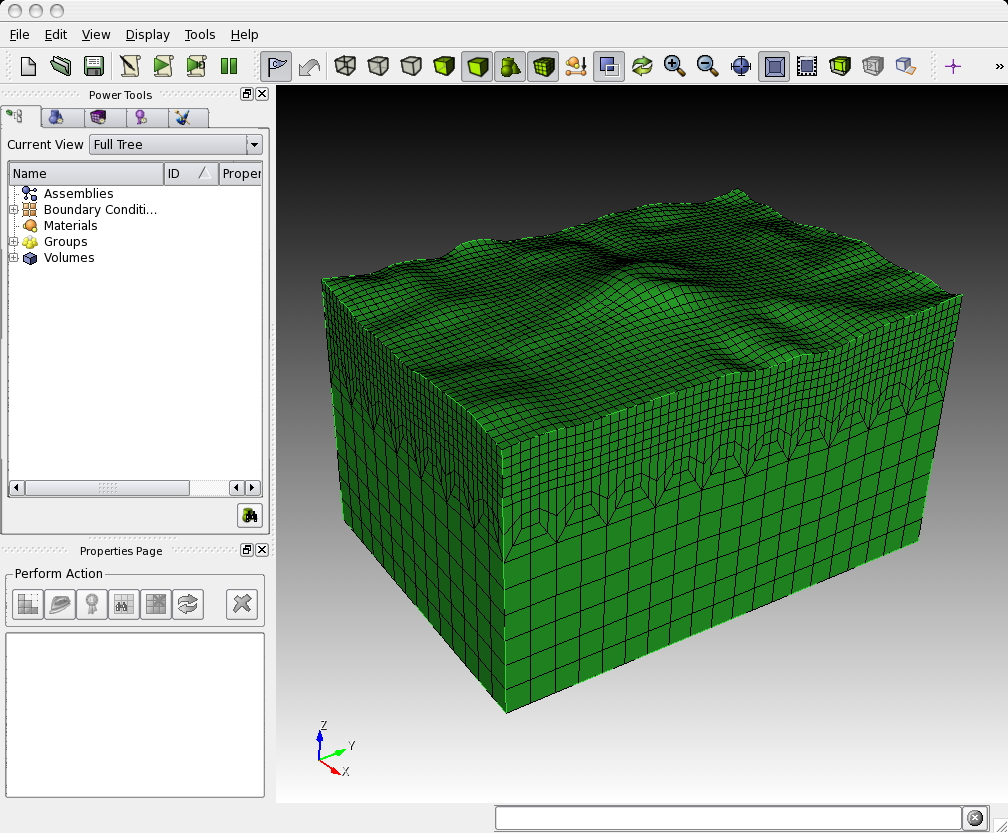
\includegraphics[width=.6\textwidth]{figures/mount-cubit.jpg}
\par\end{centering}

\caption{Example of the graphical user interface of CUBIT. The hexahedral mesh shown in the main display consists of a hexahedral discretization of a single volume with topography.}

\label{fig:mount.cubit}
\end{figure}

The basic steps in creating a load-balanced, partitioned mesh with CUBIT are:
\begin{description}
\item [1.] setting up a hexahedral mesh with CUBIT,
\item [2.] exporting the CUBIT mesh into a SPECFEM3D file format and
\item [3.] partitioning the SPECFEM3D mesh files for a chosen number of cores.
\end{description}

Examples are provided in the SPECFEM3D package in the subdirectory \texttt{examples/}. We strongly encourage you to contribute your own example to this package by contacting the CIG Computational Seismology Mailing List  \url{cig-seismo@geodynamics.org}.


\subsection{Creating the Mesh with CUBIT}

For the installation and handling of the CUBIT meshing tool suite, please refer to the CUBIT user manual and documentation.
In order to give you a basic understanding of how to use CUBIT for our purposes, examples are provided in the SPECFEM3D package in the subdirectory \texttt{examples/}:
\begin{description}
\item [{\texttt{homogeneous\_halfspace}}] Creates a single block model and assigns elastic material parameters.
\item [{\texttt{layered\_halfspace}}]  Combines two different, elastic material volumes and creates a refinement layer between the two. This example can be compared for validation against the solutions provided in subdirectory ~\\
\texttt{VALIDATION\_3D\_SEM\_SIMPLER\_LAYER\_SOURCE\_DEPTH/}.
\item [{\texttt{waterlayered\_halfspace}}] Combines an acoustic and elastic material volume as in a schematic marine survey example.
\item [{\texttt{tomographic\_model}}] Creates a single block model whose material properties will have to be read in from a tomographic model file during the databases creation by \texttt{xgenerate\_databases}.
\end{description}

\begin{figure}[htbp]
\noindent \begin{centering}
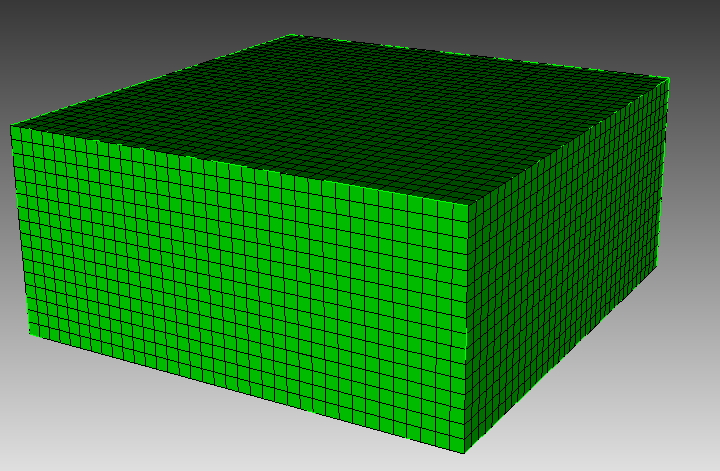
\includegraphics[width=.45\textwidth]{figures/example-homogeneous.jpg}
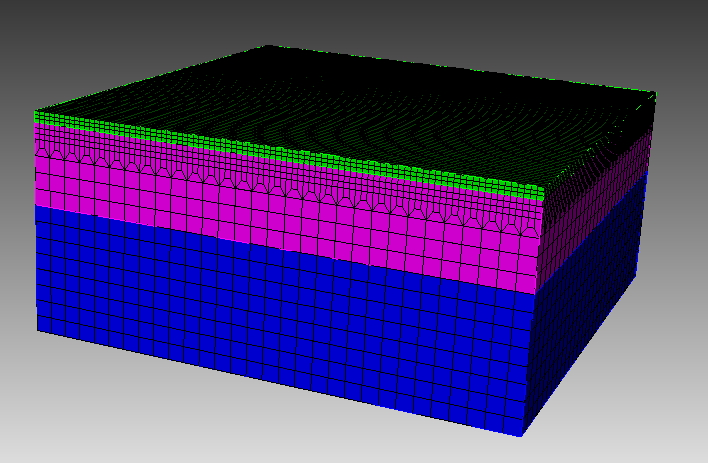
\includegraphics[width=.45\textwidth]{figures/example-2layers.jpg} \\
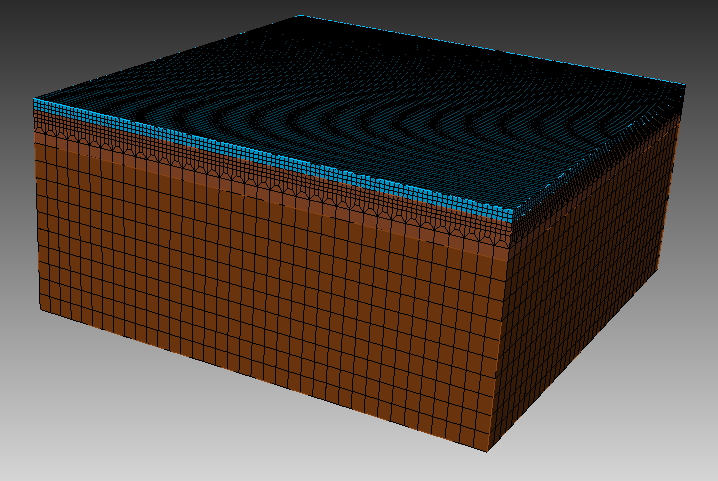
\includegraphics[width=.45\textwidth]{figures/example-water.jpg}
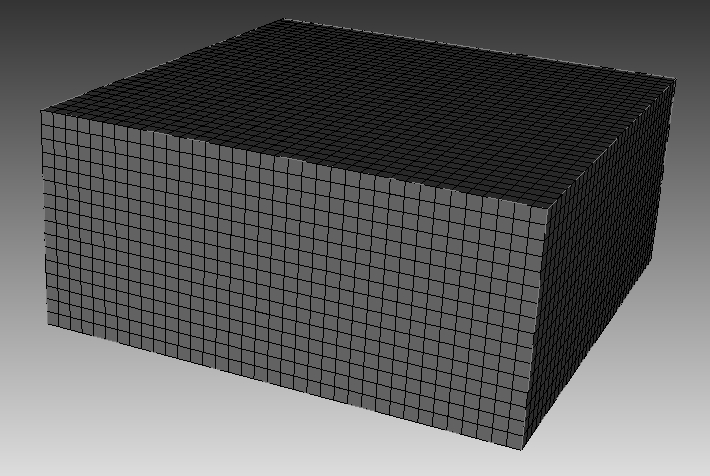
\includegraphics[width=.45\textwidth]{figures/example-tomo.jpg}
\par\end{centering}

\caption{Screenshots of the CUBIT examples provided in subdirectory  \texttt{examples/}: homogeneous halfspace (top-left), layered halfspace (top-right), water layered halfspace (bottom-left) and tomographic model (bottom-right).}

\label{fig:examples.cubit}
\end{figure}


In each example subdirectory you will find a \texttt{README} file, which explains in a step-by-step tutorial the workflow for the example.
Please feel free to contribute your own example to this package by contacting the CIG Computational Seismology Mailing List  \url{cig-seismo@geodynamics.org}.


\subsection{Exporting the Mesh with \texttt{cubit2specfem3d.py} }
\label{subsec:Exporting-the-Mesh}

Once the geometric model volumes in CUBIT are meshed, you prepare the model for exportation with the definition of material blocks and boundary surfaces. Thus, prior to exporting the mesh, you need to define blocks specifying the materials and absorbing boundaries in CUBIT.
This process could be done automatically using the script \texttt{boundary\_definition.py} if the mesh meets some conditions or manually, following the block convention:

\begin{description}
\item [material\_name] Each material should have a specific block defined by a unique name. The name convention of the material is to start with either 'elastic' or 'acoustic'. It must be then followed by a unique identifier, e.g. 'elastic 1', 'elastic 2', etc.
The additional attributes to the block define the material description.

For an elastic material:
\begin{description}
\item [material\_id] An integer value which is unique for this material.
\item [Vp] P-wave speed of the material (given in m/s).
\item [Vs] S-wave speed of the material (given in m/s).
\item [rho] density of the material (given in kg/m$^3$).
\item [Q] quality factor to use in case of a simulation with attenuation turned on. It should be between 1 and 9000. In case no attenuation information is available, it can be set to zero. Please note that your Vp- and Vs-speeds are given for a reference frequency. To change this reference frequency, you change the value of
\texttt{ATTENUATION\_f0\_REFERENCE} in the main constants file \texttt{constants.h} found in subdirectory \texttt{src/shared/}.
\item [anisotropic\_flag] Flag describing the anisotropic model to use in case an anisotropic simulation should be conducted. See the file \texttt{model\_aniso.f90} in subdirectory \texttt{src/generate\_databases/} for an implementation of the anisotropic models. In case no anisotropy is available, it can be set to zero.
\end{description}
Note that this material block has to be defined using all the volumes which belong to this elastic material. For volumes belonging to another, different material, you will need to define a new material block.

For an acoustic material:
\begin{description}
\item [material\_id] An integer value which is unique for this material.
\item [Vp] P-wave speed of the material (given in m/s).
\item [0] S-wave speed of the material is ignored.
\item [rho] density of the material (given in kg/m$^3$).
\end{description}


\item [face\_topo] Block definition for the surface which defines the free surface (which can have topography). The name of this block must be 'face\_topo', the block has to be defined using all the surfaces which constitute the complete free surface of the model.

\item [face\_abs\_xmin] Block definition for the faces on the absorbing boundaries, one block for each surface with x=Xmin.
\item [face\_abs\_xmax] Block definition for the faces on the absorbing boundaries, one block for each surface with x=Xmax.
\item [face\_abs\_ymin] Block definition for the faces on the absorbing boundaries, one block for each surface with y=Ymin.
\item [face\_abs\_ymax] Block definition for the faces on the absorbing boundaries, one block for each surface with y=Ymax.
\item [face\_abs\_bottom] Block definition for the faces on the absorbing boundaries, one block for each surface with z=bottom.
\end{description}


\begin{figure}[htbp]
\noindent \begin{centering}
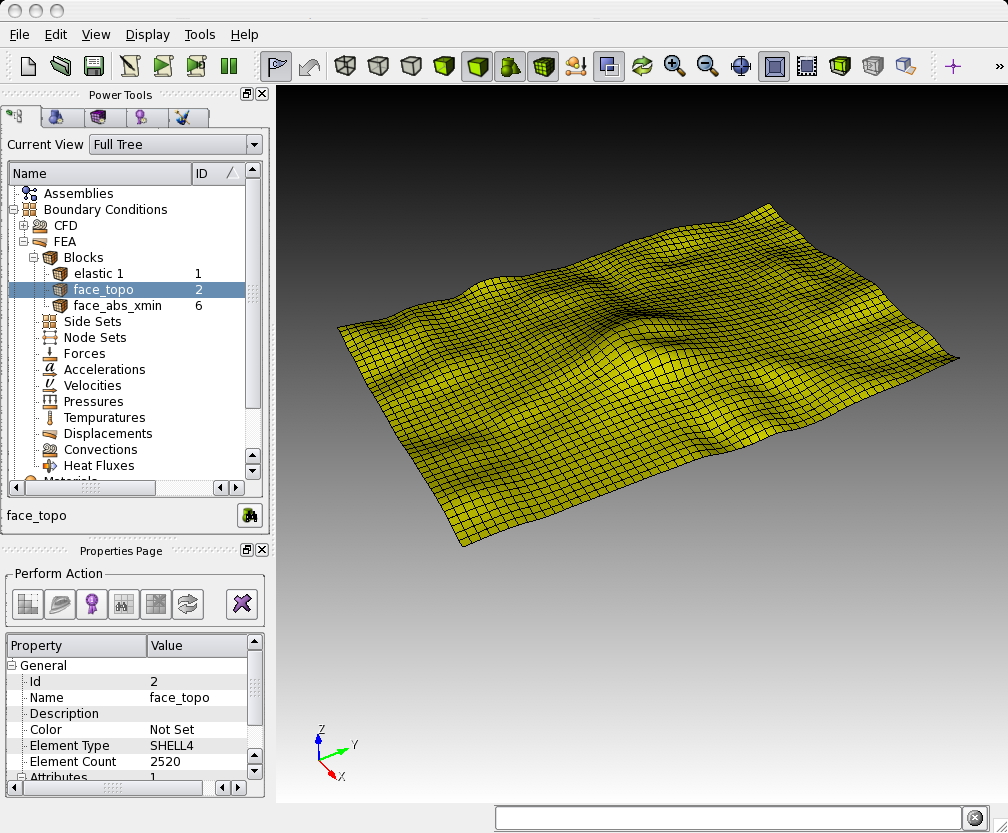
\includegraphics[width=.45\textwidth]{figures/mount-surface.jpg}
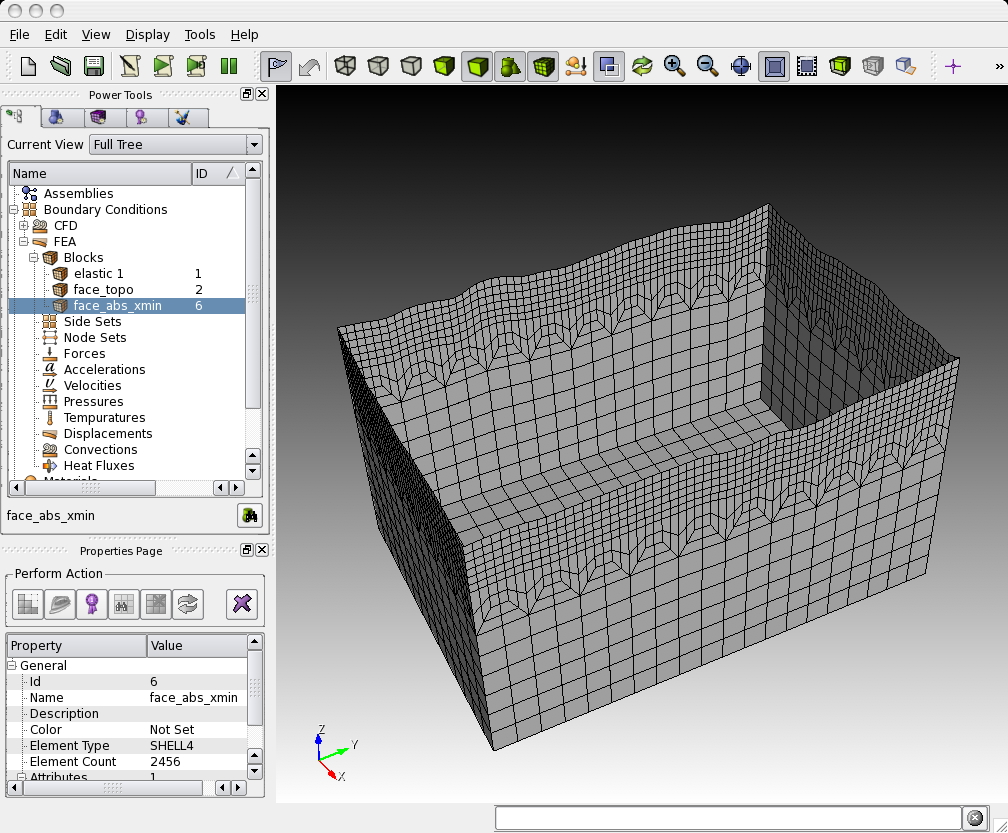
\includegraphics[width=.45\textwidth]{figures/mount-abs.jpg}
\par\end{centering}

\caption{Example of the block definitions for the free surface 'face\_topo' (left) and the absorbing boundaries, defined in a single block 'face\_abs\_xmin' (right) in CUBIT.}

\label{fig:mount.abs}
\end{figure}

Optionally, instead of specifying for each surface at the boundaries a single block like mentioned above, you can also specify a single block for all boundary surfaces and name it as one of the absorbing blocks above, e.g. 'face\_abs\_xmin'.

After the block definitions are done, you export the mesh using the script \texttt{cubit2specfem3d.py} provided in each of the example directories. If the export was successful, you should find the following files in a subdirectory \texttt{MESH/}:

\begin{description}
\item [nummaterial\_velocity\_file] Defines the material properties. For fully defined materials, the formats is:
\begin{lyxcode}
\texttt{domain\_ID} \texttt{material\_ID}  \texttt{rho}  \texttt{vp}  \texttt{vs}  \texttt{Q}  \texttt{anisotropy\_flag}
\end{lyxcode}
where
\texttt{domain\_ID} is 1 for acoustic or 2 for elastic materials, \texttt{material\_ID} a unique identifier,  \texttt{rho} the density in $kg \, m^{-3}$,  \texttt{vp} the P-wave speed in $m \, s^{-1}$, \texttt{vs}  the S-wave speed in $m \, s^{-1}$, \texttt{Q} the quality factor and \texttt{anisotropy\_flag} an identifier for anisotropic models.
For a tomographic model, the material definition format is:
\begin{lyxcode}
\texttt{domain\_ID} \texttt{material\_ID}  \texttt{tomography}  \texttt{name}
\end{lyxcode}
where
\texttt{domain\_ID} is 1 for acoustic or 2 for elastic materials, \texttt{material\_ID} a negative, unique identifier, \texttt{tomography} keyword for tomographic material definition and \texttt{name} the name of the tomography file. The name is not used so far, rather change the filename defined in the file \texttt{model\_tomography.f90} located in the
\texttt{src/generate\_databases/} directory.
\item [materials\_file] Contains the material associations for each element.
\item [nodes\_coords\_file] Contains the point locations in Cartesian coordinates of the mesh element corners.
\item [mesh\_file] Contains the mesh element connectivity.
\item [free\_surface\_file] Contains the free surface connectivity.
\item [absorbing\_surface\_file\_xmax] Contains the surface connectivity of the absorbing boundary surface at the Xmax.
\item [absorbing\_surface\_file\_xmin] Contains the surface connectivity of the absorbing boundary surface at the Xmin.
\item [absorbing\_surface\_file\_ymax] Contains the surface connectivity of the absorbing boundary surface at the Ymax.
\item [absorbing\_surface\_file\_ymin] Contains the surface connectivity of the absorbing boundary surface at the Ymin.
\item [absorbing\_surface\_file\_bottom] Contains the surface connectivity of the absorbing boundary surface at the bottom.
\end{description}

These mesh files are needed as input files for the partitioner  \texttt{xdecompose\_mesh\_SCOTCH}
to load-balance the mesh. Please see the next section for further details.


\subsubsection*{Checking the mesh quality}
The quality of the mesh may be inspected more precisely based upon the serial code
in the file  ~\\
\texttt{check\_mesh\_quality\_CUBIT\_Abaqus.f90}. 
Running this code is optional because no information needed by the
solver is generated.


Prior to running and compiling this code, you have to export your mesh in CUBIT to an ABAQUS (.inp) format.
You also have to determine a number of parameters of your mesh, such as the number of nodes and number of elements
and modify the header of the \texttt{check\_mesh\_quality\_CUBIT\_Abaqus.f90} source file. Then, 
in the directory \texttt{src/check\_mesh\_quality\_CUBIT\_Abaqus}, type
\begin{lyxcode}
{\small ./compile\_all.csh}{\small \par}
\end{lyxcode}
and use
\begin{lyxcode}
{\small xcheck\_mesh\_quality\_CUBIT\_Abaqus}{\small \par}
\end{lyxcode}
to generate an AVS output file (\texttt{\small AVS\_meshquality.inp}
in AVS UCD format) or OpenDX output file (\texttt{\small DX\_meshquality.}~\\
\texttt{\small dx}) that can be used to investigate mesh quality,
e.g, skewness of elements and a Gnuplot histogram (\texttt{\small mesh\_quality\_}~\\
\texttt{\small histogram.txt}) that can be plotted with gnuplot (type
`\texttt{\small gnuplot plot\_mesh\_quality\_histogram.gnu}'). The
histogram is also printed to the screen. If you want to start designing
your own meshes, this tool is useful for viewing your creations. You
are striving for meshes with elements with `cube-like' dimensions,
e.g., the mesh should contain no very elongated or skewed elements.


\subsection{Partitioning the Mesh with \texttt{xdecompose\_mesh\_SCOTCH}}


The SPECFEM3D software package performs large scale simulations in a parallel 'Single Process Multiple Data' way.
The spectral-element mesh created with CUBIT needs to be distributed on the processors. This partitioning is executed once and for all prior to
the execution of the solver so it is referred to as a static mapping.

An efficient partitioning is important because it leverages the overall running time of the application.
It amounts to balance the number of elements in each slice while minimizing the communication costs
resulting from the placement of adjacent elements on different processors. \texttt{decompose\_mesh\_SCOTCH} depends on the Scotch library
which provides efficent static mapping, graph and mesh partitioning routines. Scotch is a free software package developed by
Fran\c {c}ois Pellegrini et al. from LaBRI and INRIA in Bordeaux, France, downloadable from the web page \url{https://gforge.inria.fr/projects/scotch/}. It is more recent than METIS, actively maintained and performs better in many cases.
\\

Prior to compiling \texttt{decompose\_mesh\_SCOTCH}, make sure you have correctly specified the path
of the Scotch library with the option \texttt{-{}-with-scotch-path} of the \texttt{configure} script.
For convenience we provide the source code of SCOTCH, which is released open source under the French CeCILL-C version 1 license,
in directory ~\\
\texttt{src/decompose\_mesh\_SCOTCH/scotch\_5.1.10b}. Please refer to file INSTALL.txt in that directory to see how to compile it.
In the future you should be able to find more recent versions at  \url{http://www.labri.fr/perso/pelegrin/scotch/scotch\_en.html} .
\\

\begin{figure}[htbp]
\noindent \begin{centering}
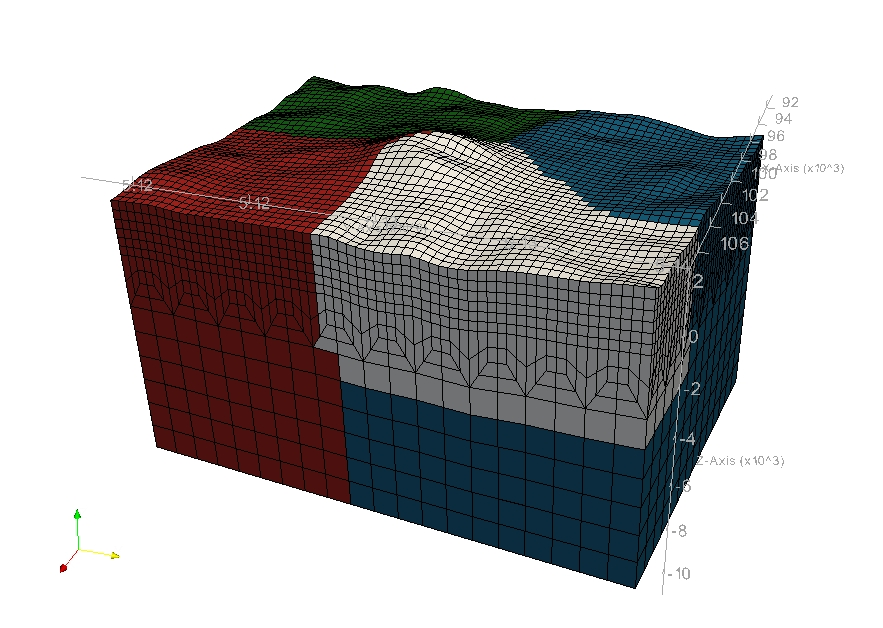
\includegraphics[width=.45\textwidth]{figures/mount-partitions.jpg}
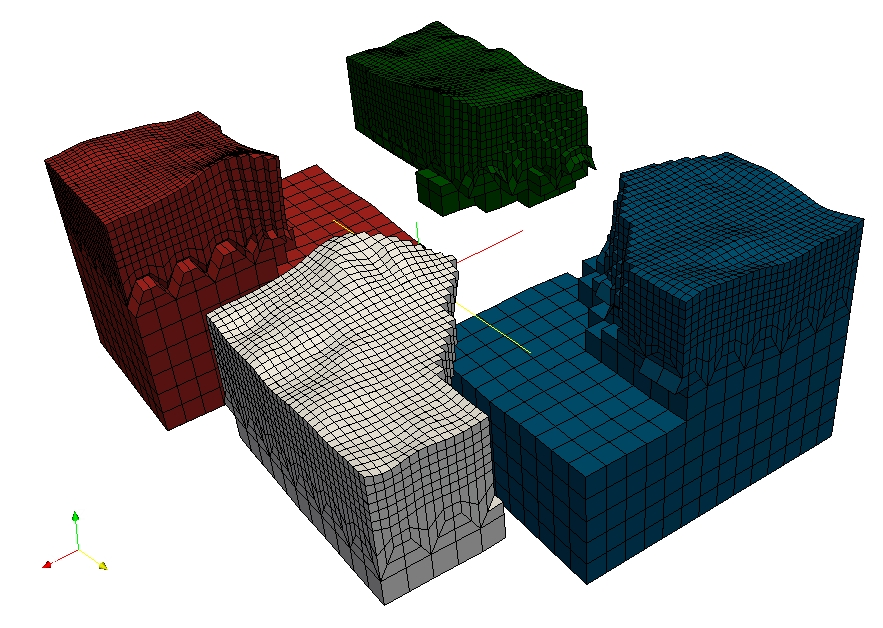
\includegraphics[width=.45\textwidth]{figures/mount-partitions2.jpg}
\par\end{centering}

\caption{Example of a mesh partitioning onto four cores. Each single core partition is colored differently. The executable \texttt{xdecompose\_mesh\_SCOTCH} can equally distribute the mesh on any arbitrary number of cores.}


\label{fig:mount.partitions}
\end{figure}

When you are ready to compile,
in the main directory type '\texttt{make decompose\_mesh\_SCOTCH}'.
If all paths and flags have been set correctly, the executable \texttt{bin/xdecompose\_mesh\_SCOTCH} should be produced.

The partitioning is done in serial for now (in the next release we will provide a parallel version of that code),
the synopsis is:
\begin{lyxcode}
./bin/xdecompose\_mesh\_SCOTCH  nparts  input\_directory output\_directory
\end{lyxcode}
where
\begin{itemize}
     \item \texttt{nparts} is the number of partitions, i.e., the number of cores for the parallel simulations,
     \item \texttt{input\_directory} is the directory which holds all the files generated by the Python script \texttt{cubit2specfem3d.py} explained in the previous Section~\ref{subsec:Exporting-the-Mesh}, e.g. \texttt{MESH/}, and
     \item \texttt{output\_directory} is the directory for the output of this partitioner which stores ACII-format files named like \texttt{proc******\_Database} for each partition. These files will be needed for creating the distributed databases, and have to reside in the directory  \texttt{LOCAL\_PATH} specified in the main \texttt{Par\_file}, e.g. in directory \texttt{in\_out\_files/DATABASES\_MPI}. Please see Chapter~\ref{cha:Creating-Distributed-Databases} for further details.
\end{itemize}
Note that all the files generated by the Python script  \texttt{cubit2specfem3d.py} must be placed in the \texttt{input\_directory} folder before running the program.

\section{\label{cha:Running-the-Mesher-Meshfem3D}Meshing with \texttt{xmeshfem3D}}

In case you successfully ran the configuration script, you are also ready to compile the internal mesher.
This is an alternative to CUBIT
for the mesh generation of relatively simple geological models. The mesher is no longer
dedicated to Southern California and more flexiblity is provided in this version of the package.

%\noindent \begin{flushleft}
%
\begin{figure}[htbp]
\noindent \begin{centering}
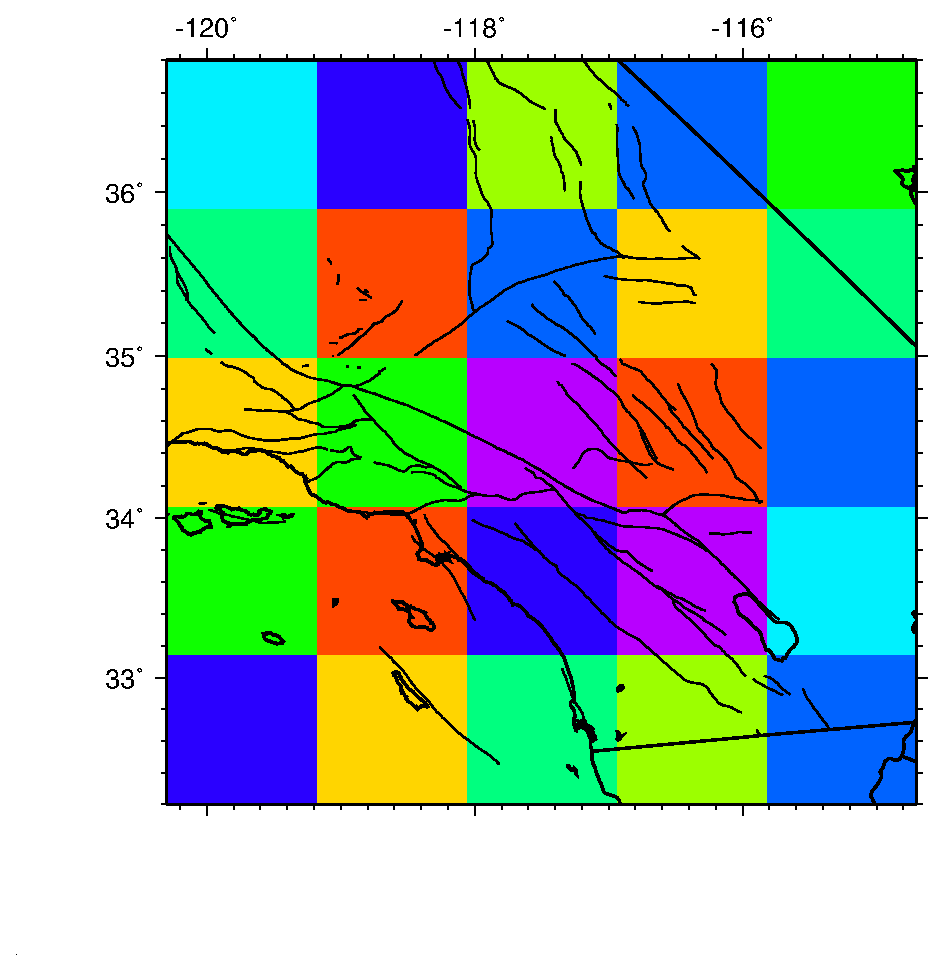
\includegraphics[scale=0.5]{figures/socal_map_mpi}
\par\end{centering}

\caption{\label{fig:For-parallel-computing}For parallel computing purposes,
the model block is subdivided in $\nprocxi\times\nproceta$ slices
of elements. In this example we use $5^{2}=25$ processors. }

\end{figure}

%\par\end{flushleft}

In the main directory type `\texttt{make meshfem3D}'. If all paths and flags
have been set correctly, the mesher should now compile and produce
the executable \texttt{bin/xmeshfem3D}. Please note that
\texttt{xmeshfem3D} must be called directly from the \texttt{bin/} directory,
as most of the binaries of the package.

Input for the mesh generation program is provided through the parameter
file \texttt{Mesh\_Par\_file}, which resides in the subdirectory \texttt{in\_data\_files/meshfem3D\_files/}.
Before running the mesher, a number of parameters need to be set in
the \texttt{Mesh\_Par\_file}. This requires a basic understanding of how
the SEM is implemented, and we encourage you to read \citet{KoVi98,KoTr99}
and \citet{KoLiTrSuStSh04}.

The mesher and the solver use UTM coordinates internally, therefore
you need to define the zone number for the UTM projection (e.g., zone
11 for Los Angeles). Use decimal values for latitude and longitude
(no minutes/seconds). These values are approximate; the mesher will
round them off to define a square mesh in UTM coordinates. When running
benchmarks on rectangular models, turn the UTM projection off by using
the flag \texttt{\small SUPPRESS\_UTM\_PROJECTION}, in which case
all `longitude' parameters simply refer to the $x$~axis, and all
`latitude' parameters simply refer to the $y$~axis. To run the mesher
for a global simulation, the following parameters need to be set in
the \texttt{Mesh\_Par\_file}:

\begin{description}
\item [{\texttt{LATITUDE\_MIN}}] Minimum latitude in the block (negative
for South).
\item [{\texttt{LATITUDE\_MAX}}] Maximum latitude in the block.
\item [{\texttt{LONGITUDE\_MIN}}] Minimum longitude in the block (negative
for West).
\item [{\texttt{LONGITUDE\_MAX}}] Maximum longitude in the block.
\item [{\texttt{DEPTH\_BLOCK\_KM}}] Depth of bottom of mesh in kilometers.
\item [{\texttt{\noun{UTM\_PROJECTION\_ZONE}}}] UTM projection zone in
which your model resides, only valid when \texttt{SUPPRESS\_UTM\_}~\\
\texttt{PROJECTION} is \texttt{.false.}.
\item [{\texttt{SUPPRESS\_UTM\_PROJECTION}}] set to be \texttt{.false.}
when your model range is specified in geographical coordinates,
and needs to be \texttt{.true.} when your model is specified in
Cartesian coordinates. \noun{UTM projection zone in which your simulation
region resides.}
\item [{\texttt{INTERFACES\_FILE }}] File which contains the description of the topography and
of the interfaces between the different layers of the model, if any.
The number of spectral elements in the vertical direction within each layer is also defined in this file.

\item [{$\nexxi$}] The number of spectral elements along one side of the
block. This number \textit{must} be 8~$\times$~a multiple of $\nprocxi$
defined below. Based upon benchmarks against semi-analytical discrete
wavenumber synthetic seismograms \citep{KoLiTrSuStSh04}, determined
that a $\nexxi=288$ run is accurate to a shortest period of roughly
2~s. Therefore, since accuracy is determined by the number of grid
points per shortest wavelength, for any particular value of $\nexxi$
the simulation will be accurate to a shortest period determined by
\begin{equation}
\mbox{shortest period (s)}=(288/\nexxi)\times2.\label{eq:shortest_period}\end{equation}
The number of grid points in each orthogonal direction of the reference
element, i.e., the number of Gauss-Lobatto-Legendre points, is determined
by \texttt{NGLLX} in the \texttt{constants.h} file. We generally use
$\mbox{\texttt{NGLLX\/}}=5$, for a total of $5^{3}=125$ points per
elements. We suggest not to change this value.
\item [{$\nexeta$}] The number of spectral elements along the other side
of the block. This number \textit{must} be 8~$\times$~a multiple
of $\nproceta$ defined below.
\item [{$\nprocxi$}] The number of processors or slices along one side
of the block (see Figure~\ref{fig:For-parallel-computing}); we must
have $\nexxi=8\times c\times\nprocxi$, where $c\ge1$ is a positive
integer.
\item [{$\nproceta$}] The number of processors or slices along the other
side of the block; we must have $\nexeta=8\times c\times\nproceta$,
where $c\ge1$ is a positive integer.
\item [{\texttt{USE\_REGULAR\_MESH}}] set to be \texttt{.true.} if you want a perfectly regular
mesh or \texttt{.false.} if you want to add doubling horizontal layers to coarsen the mesh. In this case, you
also need to provide additional information by setting up the next three parameters.
\item [{\texttt{NDOUBLINGS}}] The number of horizontal doubling layers. Must be set to \texttt{1} or \texttt{2}
if \texttt{USE\_REGULAR\_MESH} is set to \texttt{.true.}.
\item [{\texttt{NZ\_DOUBLING\_1}}] The position of the first doubling layer (only interpreted
if \texttt{USE\_REGULAR\_MESH} is set to \texttt{.true.}).
\item [{\texttt{NZ\_DOUBLING\_2}}] The position of the second doubling layer (only interpreted
if \texttt{USE\_REGULAR\_MESH} is set to \texttt{.true.} and if \texttt{NDOUBLINGS} is set to \texttt{2}).
\item [{\texttt{CREATE\_ABAQUS\_FILES}}] Set this flag to \texttt{.true.} to save Abaqus FEA \url{www.simulia.com}
mesh files for subsequent viewing. Turning the flag on generates files in the \texttt{LOCAL\_PATH} directory.
See Section~\ref{sec:Mesh-graphics} for a discussion of mesh viewing features.
\item [{\texttt{CREATE\_DX\_FILES}}] Set this flag to \texttt{.true.} to save OpenDX \url{www.opendx.org}
mesh files for subsequent viewing.
\item [{\texttt{LOCAL\_PATH}}] Directory in which the partitions generated
by the mesher will be written. Generally one uses a directory on the
local disk of the compute nodes, although on some machines these partitions
are written on a parallel (global) file system (see also the earlier
discussion of the \texttt{LOCAL\_PATH\_IS\_ALSO\_GLOBAL} flag in Chapter~\ref{cha:Getting-Started}).
The mesher generates the necessary partitions in parallel, one set
for each of the $\nprocxi\times\nproceta$ slices that constitutes
the mesh (see Figure~\ref{fig:For-parallel-computing}). After the
mesher finishes, you can log in to one of the compute nodes and view
the contents of the \texttt{LOCAL\_PATH} directory to see the
files generated by the mesher.
These files will be needed for creating the distributed databases, and have to reside in the directory  \texttt{LOCAL\_PATH} specified in the main \texttt{Par\_file}, e.g. in directory \texttt{in\_out\_files/DATABASES\_MPI}. Please see Chapter~\ref{cha:Creating-Distributed-Databases} for further details.
\item [{\texttt{NMATERIALS}}] The number of different materials in your model. In the following lines, each material needs to be defined as :
\begin{lyxcode}
\texttt{material\_ID}  \texttt{rho}  \texttt{vp}  \texttt{vs}  \texttt{Q}  \texttt{anisotropy\_flag} \texttt{domain\_ID}
\end{lyxcode}
where
\begin{itemize}
     \item \texttt{Q}           : quality factor (0=no attenuation)
     \item \texttt{anisotropy\_flag}  : 0=no anisotropy / 1,2,.. check with implementation in \texttt{aniso\_model.f90}
     \item \texttt{domain\_id}        : 1=acoustic / 2=elastic
\end{itemize}
\item [{\texttt{NMATERIALS}}] The number of regions in the mesh.
In the following lines, because the mesh is regular or 'almost regular', each region is defined as :
\begin{lyxcode}
  \texttt{XI\_begin}  \texttt{XI\_end}  \texttt{ETA\_begin}  \texttt{ETA\_end}  \texttt{material\_ID}
\end{lyxcode}
\end{description}

The \texttt{INTERFACES\_FILE} parameter of \texttt{Mesh\_Par\_File} defines the file which contains the settings of the topography grid and of the interfaces grids. Topography is defined as a set of elevation values on a regular 2D grid. It is also possible to
define interfaces between the layers of the model in the same way.
The file needs to define several parameters:
\begin{itemize} 
\item The number of interfaces, including the topography. This needs to be set at the first line. Then, from the bottom
to the top of the model, you need to define the grids with: 
\item \texttt{SUPPRESS\_UTM\_PROJECTION} flag as described previously, 
\item number of points along $x$ and $y$ direction (NXI and NETA), 
\item minimal $x$ and $y$ coordinates (LONG\_MIN and LAT\_MIN), 
\item spacing between points along $x$ and $y$ (SPACING\_XI and SPACING\_ETA) and 
\item the name of the file which contains the elevation values (in $y$.$x$ increasing order). 
\end{itemize}
At the end of this file, you simply need to set the number of spectral elements in the vertical direction for each layer. We provide a few models in the {\texttt{examples/}} directory.  \\

Finally, depending on your system, you might need to provide a file that tells MPI what compute nodes
to use for the simulations. The file must have a number of entries
(one entry per line) at least equal to the number of processors needed
for the run. A sample file is provided in the file \texttt{mymachines}.
This file is not used by the mesher or solver, but is required by
the \texttt{go\_mesher} and \texttt{go\_solver} default job submission
scripts. See Chapter~\ref{cha:Scheduler} for information about running
the code on a system with a scheduler, e.g., LSF.

Now that you have set the appropriate parameters in the \texttt{Mesh\_Par\_file}
and have compiled the mesher, you are ready to launch it! This is
most easily accomplished based upon the \texttt{go\_mesher} script.
When you run on a PC cluster, the script assumes that the nodes are
named n001, n002, etc. If this is not the case, change the \texttt{tr
-d `n'} line in the script. You may also need to edit the last command
at the end of the script that invokes the \texttt{mpirun} command.
See Chapter~\ref{cha:Scheduler} for information about running the
code on a system with a scheduler, e.g., LSF.

Mesher output is provided in the \texttt{in\_out\_files/OUTPUT\_FILES} directory
in \texttt{output\_mesher.txt}; this file provides lots of details
about the mesh that was generated. Please note that the mesher suggests a time step \texttt{DT} to run
the solver with. The mesher output file also contains a table about the quality of the mesh to indicate
possible problems with the distortions of elements. 
Alternatively, output can be directed
to the screen instead by uncommenting a line in \texttt{constants.h}:
\begin{lyxcode}
!~uncomment~this~to~write~messages~to~the~screen~

!~integer,~parameter~::~IMAIN~=~ISTANDARD\_OUTPUT
\end{lyxcode}


\chapter{\label{cha:Creating-Distributed-Databases}Creating the Distributed Databases}

After using \texttt{xmeshfem3D} or \texttt{xdecompose\_mesh\_SCOTCH}, the next step in the workflow is to compile \texttt{xgenerate\_databases}. This program is going to create all the missing information needed by the SEM solver.

\begin{figure}[htbp]
\noindent \begin{centering}
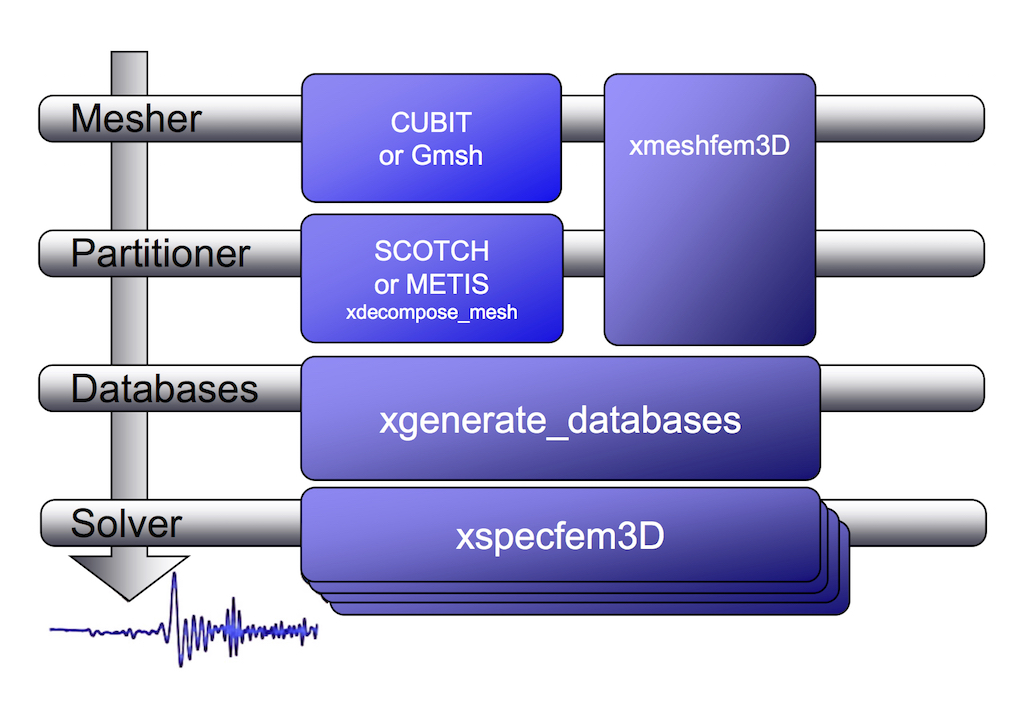
\includegraphics[width=.6\textwidth]{figures/workflow.jpg}
\par\end{centering}

\caption{Schematic workflow for a SPECFEM3D simulation. The exectable \texttt{xgenerate\_databases} creates the GLL mesh points and assigns specific model parameters.}

\label{fig:workflow.databases}
\end{figure}


In the main directory type '\texttt{make generate\_databases}'. Input for the program is provided through
the main parameter file \texttt{Par\_file}, which resides in the subdirectory \texttt{in\_data\_files/}. Please note that
\texttt{xgenerate\_databases} must be called directly from the \texttt{bin/} directory, as most of the binaries of the package.


\section{\label{cha:Main-Parameter}Main parameter file \texttt{Par\_file}}

Before running \texttt{xgenerate\_databases}, a number of parameters need to be set in the main parameter \texttt{Par\_file}
located in the subdirectory \texttt{in\_data\_files/}:

\begin{description}
\item [{\texttt{SIMULATION\_TYPE}}] is set to 1 for forward simulations,
2 for adjoint simulations (see Section \ref{sec:Adjoint-simulation-finite})
and 3 for kernel simulations (see Section \ref{sec:Finite-Frequency-Kernels}).
\item [{\texttt{SAVE\_FORWARD}}] is only set to \texttt{.true.} for a forward
simulation with the last frame of the simulation saved, as part of
the finite-frequency kernel calculations (see Section \ref{sec:Finite-Frequency-Kernels}).
For a regular forward simulation, leave \texttt{SIMULATION\_TYPE}
and \texttt{SAVE\_FORWARD} at their default values.
\item [{\texttt{\noun{UTM\_PROJECTION\_ZONE}}}] UTM projection zone in
which your model resides, only valid when \texttt{SUPPRESS\_UTM\_}~\\
\texttt{PROJECTION} is \texttt{.false.}.
\item [{\texttt{SUPPRESS\_UTM\_PROJECTION}}] set to be \texttt{.false.}
when your model range is specified in the geographical coordinates,
and needs to be \texttt{.true.} when your model is specified in a
cartesian coordinates. \noun{UTM projection zone in which your simulation
region resides.}
\item [{\texttt{NPROC}}] The number of MPI processors, each one is assigned one slice of the whole mesh.
\item [{\texttt{NSTEP}}] The number of time steps of the simulation. This controls the
length of the numerical simulation, i.e., twice the number of time steps
requires twice as much CPU time. This feature is not used at the time
of generating the distributed databases but is required for the solver, i.e., you may change this
parameter after running  \texttt{xgenerate\_databases}.
\item [{\texttt{DT}}] The length of each time step in seconds.
This feature is not used at the time of generating the distributed databases but is required for the solver.
Please see also Section~\ref{cha:Choosing-the-Time-Step} for further details.
\item [{\texttt{OCEANS}}] Set to \texttt{.true.} if the effect of the oceans
on seismic wave propagation should be incorporated based upon the
approximate treatment discussed in \citet{KoTr02b}. This feature
is inexpensive from a numerical perspective, both in terms of memory
requirements and CPU time. This approximation is accurate at periods
of roughly 20~s and longer. At shorter periods the effect of water
phases/reverberations is not taken into account, even when the flag
is on.
%obsolete...
%\item [{\texttt{TOPOGRAPHY}}] Set to \texttt{.true.} if topography and
%bathymetry should be incorporated based upon model ETOPO5 \citep{Etopo5}.
%This feature adds no cost to the simulation.
\item [{\texttt{ATTENUATION}}] Set to \texttt{.true.} if attenuation should
be incorporated. Turning this feature on increases the memory requirements
significantly (roughly by a factor of~1.5), and is numerically fairly
expensive. See \citet{KoTr99,KoTr02a} for a discussion on the implementation
of attenuation based upon standard linear solids.
Please note that the Vp- and Vs-velocities of your model are given for a reference frequency.
To change this reference frequency, you change the value of
\texttt{ATTENUATION\_f0\_REFERENCE} in the main constants file \texttt{constants.h} found in subdirectory \texttt{src/shared/}.
\item [{\texttt{USE\_OLSEN\_ATTENUATION}}] Set to \texttt{.true.} if you
want to use the attenuation model that scaled from the S-wave speed model
using Olsen's empirical relation (see \citet{OlDaBr03}).
\item [{\texttt{ANISOTROPY}}] Set to \texttt{.true.} if you
want to use an anisotropy model. Please see the file \texttt{model\_aniso.f90} in subdirectory \texttt{src/generate\_databases/} for the current implementation of anisotropic models.
\item [{\texttt{ABSORBING\_CONDITIONS}}] Set to \texttt{.true.} to turn
on Clayton-Enquist absorbing boundary conditions (see \citet{KoTr99}).
%obsolete...
%\item [{\texttt{RECORD\_LENGTH\_IN\_MINUTES}}] Choose the desired record
%length of the synthetic seismograms (in minutes). This controls the
%length of the numerical simulation, i.e., twice the record length
%requires twice as much CPU time. This feature is not used at the time
%of meshing but is required for the solver, i.e., you may change this
%parameter after running \texttt{xgenerate\_databases}.
\item [{\texttt{MOVIE\_SURFACE}}] Set to \texttt{.false.}, unless you want
to create a movie of seismic wave propagation on the Earth's surface.
Turning this option on generates large output files. See Section \ref{sec:Movies}
for a discussion on the generation of movies. This feature is only relevant for the solver.
\item [{\texttt{MOVIE\_VOLUME}}] Set to \texttt{.false.}, unless you want
to create a movie of seismic wave propagation in the Earth's interior.
Turning this option on generates huge output files. See Section \ref{sec:Movies}
for a discussion on the generation of movies. This feature is only relevant for the solver.
\item [{\texttt{NTSTEP\_BETWEEN\_FRAMES}}] Determines the number of timesteps
between movie frames. Typically you want to save a snapshot every
100 timesteps. The smaller you make this number the more output will
be generated! See Section \ref{sec:Movies} for a discussion on the
generation of movies. This feature is only relevant for the solver.
\item [{\texttt{CREATE\_SHAKEMAP}}] Set this flag to \texttt{.true.} to
create a ShakeMap\textregistered, i.e., a peak ground velocity map
of the maximum absolute value of the two horizontal components of the velocity vector.
\item [{\texttt{SAVE\_DISPLACEMENT}}] Set this flag to \texttt{.true.}
if you want to save the displacement instead of velocity for the movie
frames.
\item [{\texttt{USE\_HIGHRES\_FOR\_MOVIES}}] Set this flag to \texttt{.true.}
if you want to save the values at all the NGLL grid points for the
movie frames.
\item [{\texttt{HDUR\_MOVIE}}] determines the half duration of the source time function for the movie simulations.
When this parameter is set to be 0, a default half duration that corresponds to the accuracy of the simulation is provided.
Otherwise, it adds this half duration to the half duration specified in the source file \texttt{CMTSOLUTION},
thus simulates longer periods to make the movie images look smoother.
\item [{\texttt{SAVE\_MESH\_FILES}}] Set this flag to \texttt{.true.} to
save ParaView \url{www.paraview.org}
mesh files for subsequent viewing. Turning the flag on generates large
(distributed) files in the \texttt{LOCAL\_PATH} directory. See Section~\ref{sec:Mesh-graphics}
for a discussion of mesh viewing features.
\item [{\texttt{LOCAL\_PATH}}] Directory in which the distributed databases
will be written. Generally one uses a directory on the
local disk of the compute nodes, although on some machines these databases
are written on a parallel (global) file system (see also the earlier
discussion of the \texttt{LOCAL\_PATH\_IS\_ALSO\_GLOBAL} flag in Chapter~\ref{cha:Getting-Started}).
\texttt{xgenerate\_databases} generates the necessary databases in parallel, one set
for each of the \texttt{NPROC} slices that constitutes
the mesh (see Figure~\ref{fig:mount.partitions} and Figure~\ref{fig:For-parallel-computing}). After
the executable finishes, you can log in to one of the compute nodes and view
the contents of the \texttt{LOCAL\_PATH} directory to see the (many)
files generated by \texttt{xgenerate\_databases}.
Please note that the \texttt{LOCAL\_PATH} directory should already contain the output files of
the partitioner, i.e. from \texttt{xdecompose\_mesh\_SCOTCH} or \texttt{xmeshfem3D}.
\item [{\texttt{NTSTEP\_BETWEEN\_OUTPUT\_INFO}}] This parameter specifies
the interval at which basic information about a run is written to
the file system (\texttt{timestamp{*}} files in the \texttt{in\_out\_files/OUTPUT\_FILES}
directory). If you have access to a fast machine, set \texttt{NTSTEP\_BETWEEN\_OUTPUT\_INFO}
to a relatively high value (e.g., at least 100, or even 1000 or more)
to avoid writing output text files too often. This feature is not
used at the time of meshing. One can set this parameter to a larger
value than the number of time steps to avoid writing output during
the run.
\item [{\texttt{NTSTEP\_BETWEEN\_OUTPUT\_SEISMOS}}] This parameter specifies
the interval at which synthetic seismograms are written in the \texttt{LOCAL\_PATH}
directory. If a run crashes, you may still find usable (but shorter
than requested) seismograms in this directory. On a fast machine set
\texttt{NTSTEP\_BETWEEN\_OUTPUT\_SEISMOS} to a relatively high value
to avoid writing to the seismograms too often. This feature is only relevant for the solver.
\item [{\texttt{PRINT\_SOURCE\_TIME\_FUNCTION}}] Turn this flag on to print
information about the source time function in the file \texttt{in\_out\_files/OUTPUT\_FILES/plot\_source\_time\_function.txt}.
This feature is only relevant for the solver.
\end{description}

%% Another file generated by \texttt{xgenerate\_databases} is the header file \texttt{OUTPUT\_FILES/values\_from\_mesher.h}.
%% This file specifies a number of constants and flags needed by the
%% solver. These values are passed statically to the solver for reasons
%% of speed. Some useful statistics about the mesh are also provided
%% in this file.

%% For a given model, set of nodes, and set of parameters in \texttt{Par\_file},
%% one only needs to run the mesher once and for all, even if one wants
%% to run several simulations with different sources and/or receivers
%% (the source and receiver information is used in the solver only).

\section{\label{cha:Choosing-the-Time-Step}Choosing the time step \texttt{DT}}

The parameter \texttt{DT} sets the length of each time step in seconds. The value of this parameter is crucial for the stability of
the spectral-element simulation. Your time step \texttt{DT} will depend on the minimum ratio between the distance $h$ of neighboring mesh points and the wave speeds $v$ defined in your model. The condition for the time step $\Delta t$ is:

\begin{lyxcode}
$\Delta t < C ~\mathrm{min}_\Omega (~ h / v ~)$
\end{lyxcode}
where $C$ is the so-called Courant number and $\Omega$ denotes the model volume.
The distance $h$ depends on the mesh element size and the number of
GLL points \texttt{NGLL} specified in the main constants file \texttt{constants.h} located in the \texttt{src/shared/} subdirectory.
The wave speed $v$ is determined based on your model's P- (or S-) wave speed values.

The database generator \texttt{xgenerate\_databases}, as well as the internal mesher \texttt{xmeshfem3D}, are trying
to evaluate the value of $\Delta t$ for empirically chosen Courant numbers $C \sim 0.3$.
If you used the mesher \texttt{xmeshfem3D} to generate your mesh, you should set the value suggested in \texttt{in\_out\_files/OUTPUT\_FILES/output\_mesher.txt} file, which is created after the mesher completed. In case you used CUBIT to create the mesh, you might use an arbitrary value when running \texttt{xgenerate\_databases} and then use the value suggested in the ~\\
\texttt{in\_out\_files/OUTPUT\_FILES/output\_mesher.txt} file after the database generation completed.
Note that the implemented Newmark time scheme uses this time step globally, thus your simulations become more expensive for very small mesh elements in high wave-speed regions. Please be aware of this restriction when constructing your mesh in Chapter~\ref{cha:Mesh-Generation}.



\chapter{\label{cha:Running-the-Solver}Running the Solver \texttt{xspecfem3D}}

Now that you have successfully generated the databases, you are ready to compile
the solver. In the main directory type `\texttt{make specfem3D}'.
Please note that \texttt{xspecfem3D} must be called directly from
the \texttt{bin/} directory, as most of the binaries of the package.

%obsolete
%For reasons of speed, the solver uses static memory allocation.
%Therefore it needs to be recompiled (type `\texttt{make clean}' and
%`\texttt{make specfem3D}') every time one reruns \texttt{xgenerate\_databases}. To compile
%the solver one needs a file created by \texttt{xgenerate\_databases} in the directory
%\texttt{OUTPUT\_FILES} called \texttt{values\_from\_mesher.h}, which
%contains parameters describing the static size of the arrays as well
%as the setting of certain flags.

The solver needs three input files in the \texttt{in\_data\_files/} directory
to run:
\begin{description}
\item [{\texttt{Par\_file}}] the main parameter file which was discussed in detail in the previous
Chapter~\ref{cha:Creating-Distributed-Databases},
\item [{\texttt{CMTSOLUTION}}] the earthquake source parameter file, and
\item [{\texttt{STATIONS}}] the stations file.
\end{description}

Most parameters in the \texttt{Par\_file}
should be set prior to running the databases generation. Only the following parameters
may be changed after running \texttt{xgenerate\_databases}:

\begin{itemize}
\item the simulation type control parameters: \texttt{SIMULATION\_TYPE}
and \texttt{SAVE\_FORWARD}
\item the time step parameters \texttt{NSTEP} and \texttt{DT}
%\item the attenuation control parameters \texttt{ATTENUATION} and \texttt{USE\_OLSEN\_ATTENUATION}
\item the absorbing boundary control parameter \texttt{ABSORBING\_CONDITIONS}
\item the movie control parameters \texttt{MOVIE\_SURFACE}, \texttt{MOVIE\_VOLUME},
and \texttt{NTSTEPS\_BETWEEN\_FRAMES}
\item the ShakeMap\textregistered option \texttt{CREATE\_SHAKEMAP}
\item the output information parameters \texttt{NTSTEP\_BETWEEN\_OUTPUT\_INFO}
and \texttt{NTSTEP\_BETWEEN\_OUTPUT\_}~\\
\texttt{SEISMOS}
\item the \texttt{PRINT\_SOURCE\_TIME\_FUNCTION} flags
\end{itemize}
Any other change to the \texttt{Par\_file} implies rerunning both
the database generator \texttt{xgenerate\_databases} and the solver \texttt{xspecfem3D}.

For any particular earthquake, the \texttt{CMTSOLUTION} file that
represents the point source may be obtained directly from the Harvard Centroid-Moment Tensor (CMT) web page \url{www.seismology.harvard.edu}.
It looks like this:

\begin{lyxcode}
{\small }%
\begin{figure}[H]
\noindent \begin{centering}
{\small 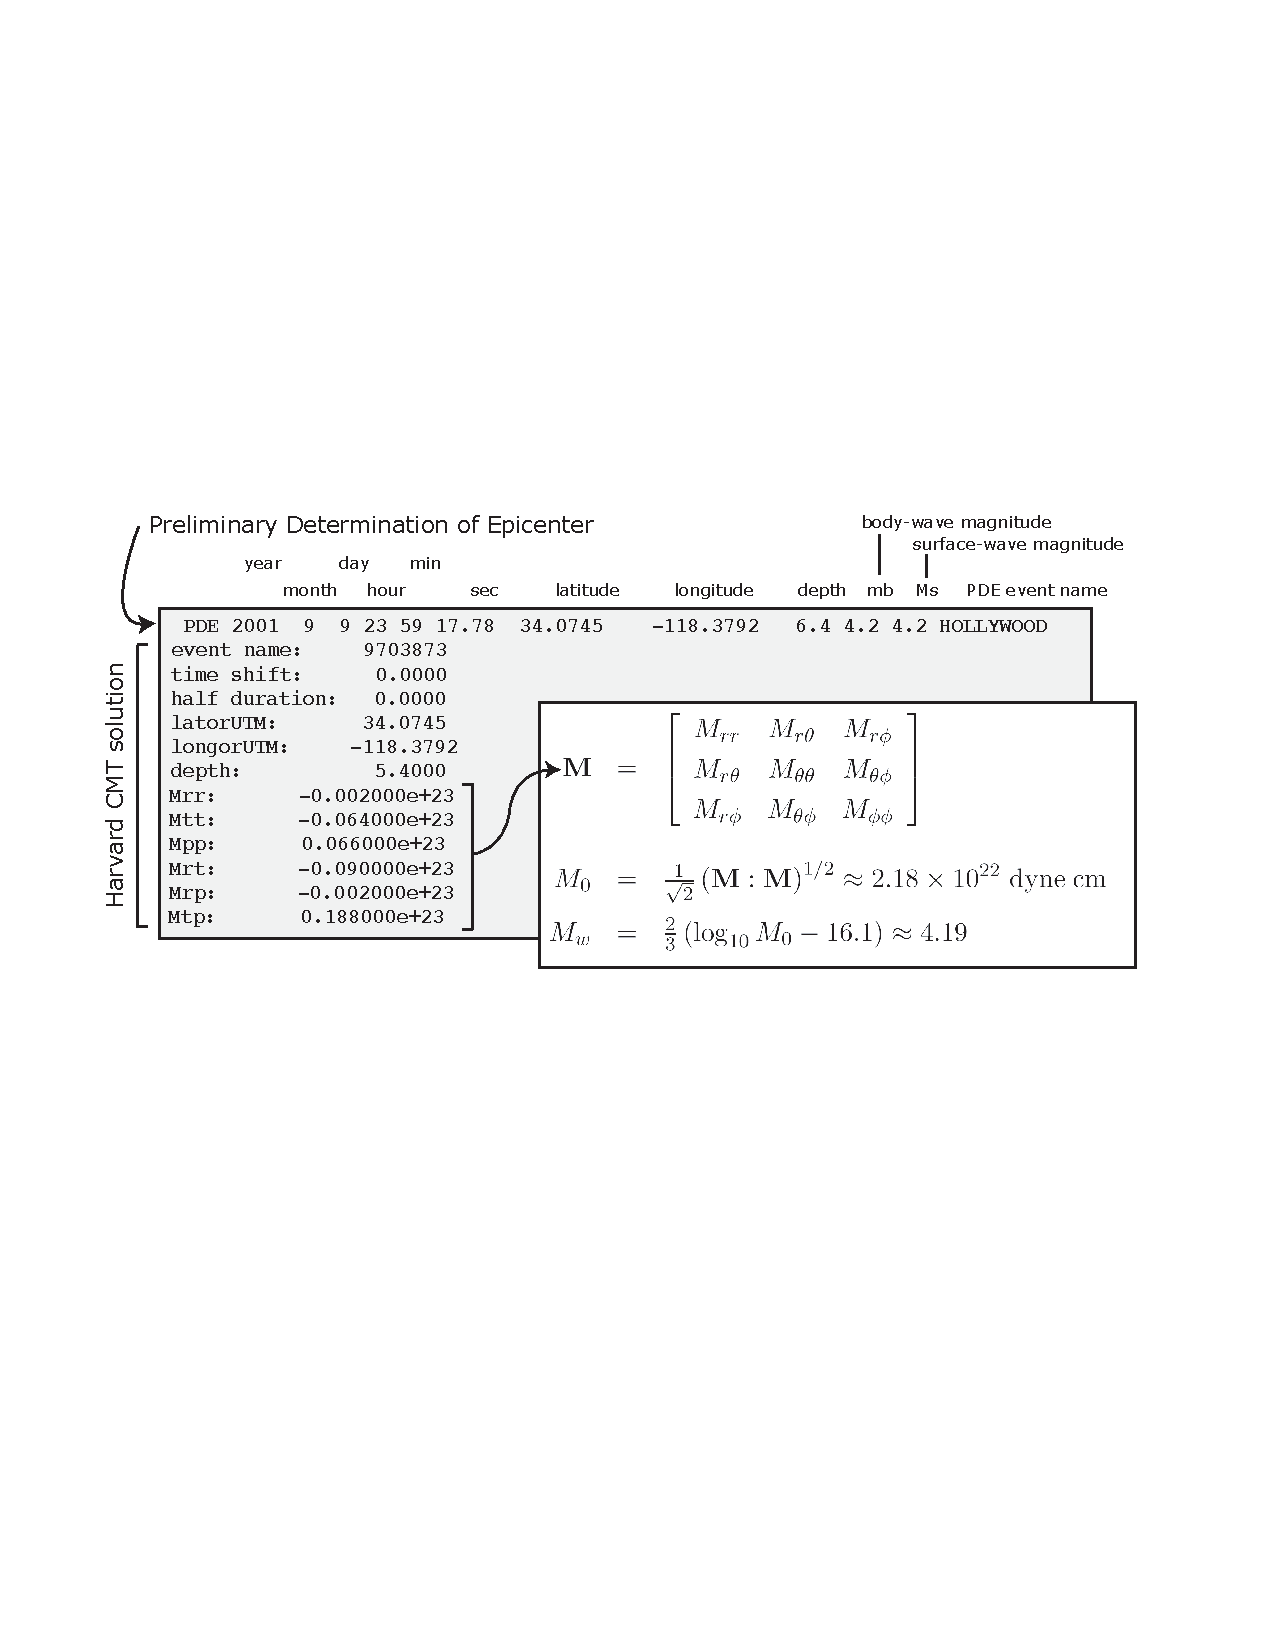
\includegraphics[width=1\textwidth]{figures/Hollywood_CMT} }
\par\end{centering}{\small \par}

\caption{\label{fig:CMTSOLUTION-file}\texttt{CMTSOLUTION} file based on the
format from the Harvard CMT catalog. \textbf{M} is the moment tensor,
$M_{0}${\small{} }is the seismic moment, and $M_{w}$ is the moment
magnitude.}

\end{figure}
{\small \par}
\end{lyxcode}
The \texttt{CMTSOLUTION} should be edited in the following way:

\begin{itemize}
\item Set the \texttt{time shift} parameter equal to $0.0$ (the solver
will not run otherwise.) The time shift parameter would simply apply
an overall time shift to the synthetics, something that can be done
in the post-processing (see Section \ref{sec:Process-data-and-syn}).
\item For point-source simulations (see finite sources, page \pageref{To-simulate-a})
we recommend setting the source half-duration parameter \texttt{half
duration} equal to zero, which corresponds to simulating a step source-time
function, i.e., a moment-rate function that is a delta function. If
\texttt{half duration} is not set to zero, the code will use a Gaussian
(i.e., a signal with a shape similar to a `smoothed triangle', as
explained in \citet{KoTr02a} and shown in Fig~\ref{fig:gauss.vs.triangle})
source-time function with half-width \texttt{half duration}. We prefer
to run the solver with \texttt{half duration} set to zero and convolve
the resulting synthetic seismograms in post-processing after the run,
because this way it is easy to use a variety of source-time functions
(see Section \ref{sec:Process-data-and-syn}). \citet{KoTr02a} determined
that the noise generated in the simulation by using a step source
time function may be safely filtered out afterward based upon a convolution
with the desired source time function and/or low-pass filtering. Use
the serial code \texttt{convolve\_source\_timefunction.f90} and the
script \texttt{convolve\_source\_timefunction.csh} for this purpose,
or alternatively use signal-processing software packages such as SAC \url{www.llnl.gov/sac}.
Type

\begin{lyxcode}
make~convolve\_source\_timefunction
\end{lyxcode}
to compile the code and then set the parameter \texttt{hdur} in \texttt{convolve\_source\_timefunction.csh}
to the desired half-duration.

\item The zero time of the simulation corresponds to the center of the triangle/Gaussian,
or the centroid time of the earthquake. The start time of the simulation
is $t=-1.5*\texttt{half duration}$ (the 1.5 is to make sure the moment
rate function is very close to zero when starting the simulation).
To convert to absolute time $t_{\mathrm{abs}}$, set

\begin{lyxcode}
$t_{\mathrm{abs}}=t_{\mathrm{pde}}+\texttt{time shift}+t_{\mathrm{synthetic}}$
\end{lyxcode}
where $t_{\mathrm{pde}}$ is the time given in the first line of the
\texttt{CMTSOLUTION}, \texttt{time shift} is the corresponding value
from the original \texttt{CMTSOLUTION} file and $t_{\mathrm{synthetic}}$
is the time in the first column of the output seismogram.

\end{itemize}
%
\begin{figure}
\noindent \begin{centering}
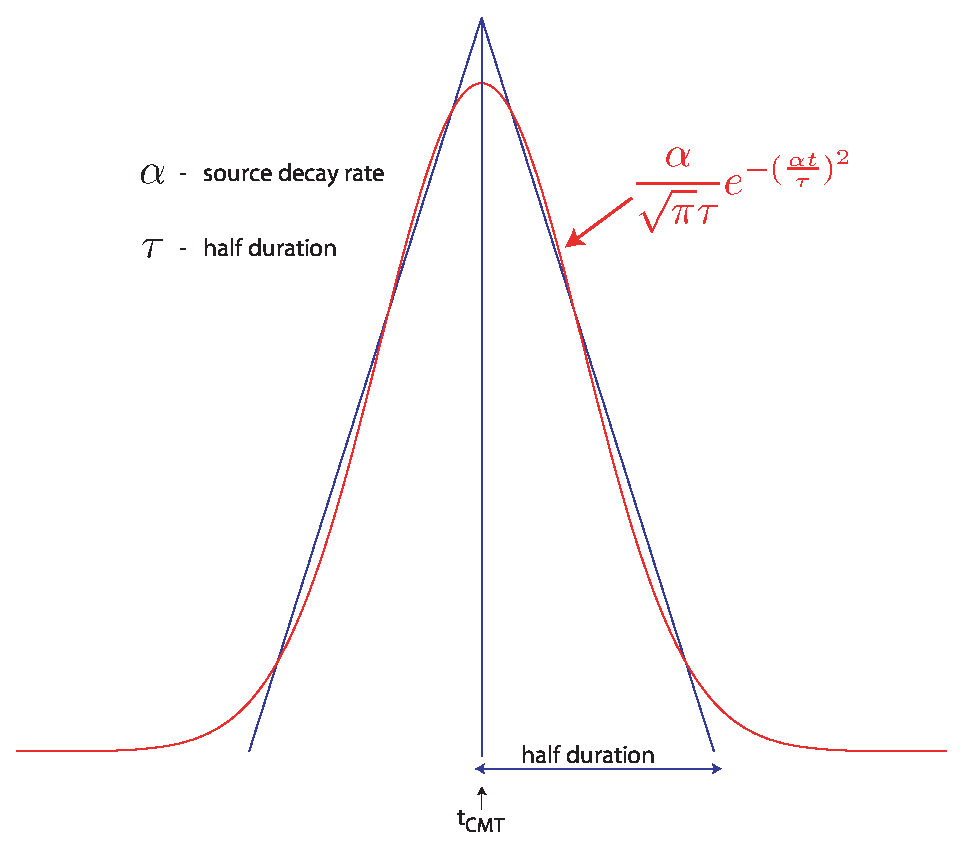
\includegraphics[width=3in]{figures/gauss_vs_triangle_mod.eps}
\par\end{centering}

\caption{Comparison of the shape of a triangle and the Gaussian function actually
used.}


\label{fig:gauss.vs.triangle}
\end{figure}


Centroid latitude and longitude should be provided in geographical
coordinates. The code converts these coordinates to geocentric coordinates~\citep{DaTr98}.
Of course you may provide your own source representations by designing
your own \texttt{CMTSOLUTION} file. Just make sure that the resulting
file adheres to the Harvard CMT conventions (see Appendix~\ref{cha:Coordinates}).
Note that the first line in the \texttt{CMTSOLUTION} file is the Preliminary Determination of Earthquakes (PDE) solution performed by the USGS NEIC, which is used as a seed for the Harvard CMT inversion. The PDE solution is based upon P waves and often gives the hypocenter of the earthquake, i.e., the rupture initiation point, whereas the CMT solution gives the `centroid location', which is the location with dominant moment release. The PDE solution is not used by our software package but must be present anyway in the first line of the file.

\label{To-simulate-a}To simulate a kinematic rupture, i.e., a finite-source
event, represented in terms of $N_{\mathrm{sources}}$ point sources,
provide a \texttt{CMTSOLUTION} file that has $N_{\mathrm{sources}}$
entries, one for each subevent (i.e., concatenate $N_{\mathrm{sources}}$
\texttt{CMTSOLUTION} files to a single \texttt{CMTSOLUTION} file).
At least one entry (not necessarily the first) must have a zero \texttt{time
shift}, and all the other entries must have non-negative \texttt{time
shift}. Each subevent can have its own half duration, latitude, longitude,
depth, and moment tensor (effectively, the local moment-density tensor).

Note that the zero in the synthetics does NOT represent the hypocentral
time or centroid time in general, but the timing of the \textit{center}
of the source triangle with zero \texttt{time shift} (Fig~\ref{fig:source_timing}).

Although it is convenient to think of each source as a triangle, in
the simulation they are actually Gaussians (as they have better frequency
characteristics). The relationship between the triangle and the gaussian
used is shown in Fig~\ref{fig:gauss.vs.triangle}. For finite fault
simulations it is usually not advisable to use a zero half duration
and convolve afterwards, since the half duration is generally fixed
by the finite fault model.

{\small }%
\begin{figure}[H]
\noindent \begin{centering}
{\small 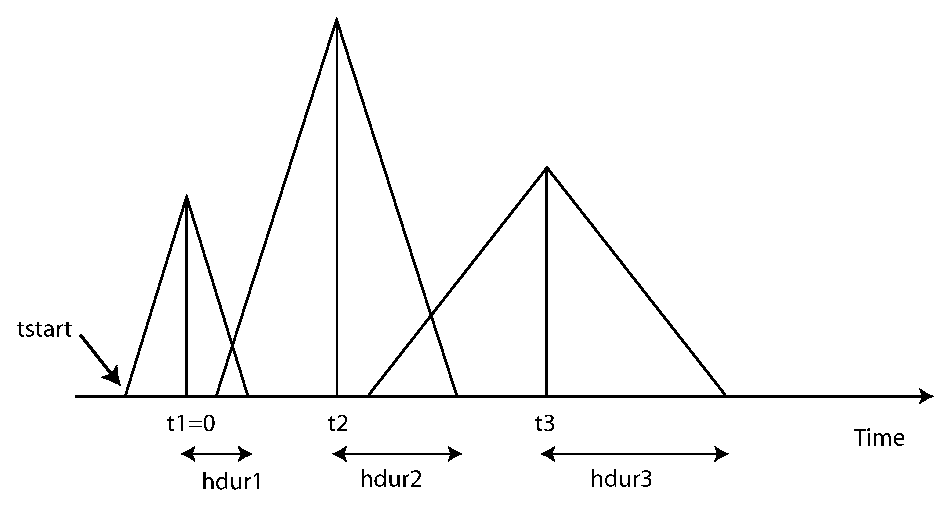
\includegraphics[width=5in]{figures/source_timing.eps} }
\par\end{centering}{\small \par}

\caption{Example of timing for three sources. The center of the first source
triangle is defined to be time zero. Note that this is NOT in general
the hypocentral time, or the start time of the source (marked as tstart).
The parameter \texttt{time shift} in the \texttt{CMTSOLUTION} file
would be t1(=0), t2, t3 in this case, and the parameter \texttt{half
duration} would be hdur1, hdur2, hdur3 for the sources 1, 2, 3 respectively.}


{\small \label{fig:source_timing} }
\end{figure}
{\small \par}

The solver can calculate seismograms at any number of stations for
basically the same numerical cost, so the user is encouraged to include
as many stations as conceivably useful in the \texttt{STATIONS} file,
which looks like this:

{\small }%
\begin{figure}[H]
\noindent \begin{centering}
{\small 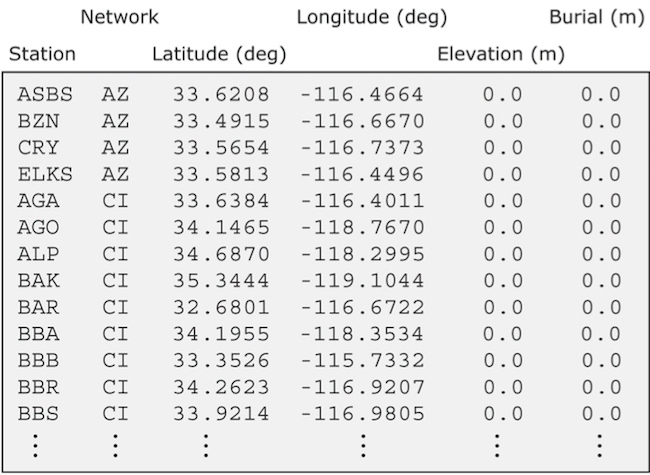
\includegraphics{figures/STATIONS_basin_explained} }
\par\end{centering}{\small \par}

\caption{Sample \texttt{STATIONS} file. Station latitude and longitude should
be provided in geographical coordinates. The width of the station
label should be no more than 32 characters (see \texttt{MAX\_LENGTH\_STATION\_NAME}
in the \texttt{constants.h} file), and the network label should be
no more than 8 characters (see \texttt{MAX\_LENGTH\_NETWORK\_NAME}
in the \texttt{constants.h} file).}

\end{figure}
{\small \par}

Each line represents one station in the following format:

\begin{lyxcode}
{\small Station~Network~Latitude~(degrees)~Longitude~(degrees)~Elevation~(m)~burial~(m)~}{\small \par}
\end{lyxcode}
The solver \texttt{xspecfem3D} filters the list of stations in file \texttt{in\_data\_files/STATIONS}
to exclude stations that are not located within the region given in
the \texttt{Par\_file} (between \texttt{LATITUDE\_MIN} and \texttt{LATITUDE\_MAX}
and between \texttt{LONGITUDE\_MIN} and \texttt{LONGITUDE\_MAX}).
The filtered file is called \texttt{in\_data\_files/STATIONS\_FILTERED}.

Solver output is provided in the \texttt{in\_out\_files/OUTPUT\_FILES} directory
in the \texttt{output\_solver.txt} file. Output can be directed to
the screen instead by uncommenting a line in \texttt{constants.h}:

\begin{lyxcode}
!~uncomment~this~to~write~messages~to~the~screen~

!~integer,~parameter~::~IMAIN~=~ISTANDARD\_OUTPUT~
\end{lyxcode}
On PC clusters the seismogram files are generally written to the local
disks (the path \texttt{LOCAL\_PATH} in the \texttt{Par\_file}) and
need to be gathered at the end of the simulation.

While the solver is running, its progress may be tracked by monitoring
the `\texttt{\small timestamp{*}}' files in the ~\\
\texttt{\small in\_out\_files/OUTPUT\_FILES} directory.
These tiny files look something like this:

\begin{lyxcode}
Time~step~\#~~~~~~~~~~10000~

Time:~~~~~108.4890~~~~~~seconds~

Elapsed~time~in~seconds~=~~~~1153.28696703911~

Elapsed~time~in~hh:mm:ss~=~~~~~0~h~19~m~13~s~

Mean~elapsed~time~per~time~step~in~seconds~=~~~~~0.115328696703911~

Max~norm~displacement~vector~U~in~all~slices~(m)~=~~~~1.0789589E-02~
\end{lyxcode}
The \texttt{\small timestamp{*}} files provide the \texttt{Mean elapsed
time per time step in seconds}, which may be used to assess performance
on various machines (assuming you are the only user on a node), as
well as the \texttt{Max norm displacement vector U in all slices~(m)}.
If something is wrong with the model, the mesh, or the source, you
will see the code become unstable through exponentially growing values
of the displacement and fluid potential with time, and ultimately
the run will be terminated by the program. You can control the rate
at which the timestamp files are written based upon the parameter
\texttt{NTSTEP\_BETWEEN\_OUTPUT\_INFO} in the \texttt{Par\_file}.

Having set the \texttt{Par\_file} parameters, and having provided
the \texttt{CMTSOLUTION} and \texttt{STATIONS} files, you are now
ready to launch the solver! This is most easily accomplished based
upon the \texttt{go\_solver} script (See Chapter \ref{cha:Scheduler}
for information about running through a scheduler, e.g., LSF). You
may need to edit the last command at the end of the script that invokes
the \texttt{mpirun} command. The \texttt{runall} script compiles and
runs both \texttt{xgenerate\_databases} and \texttt{xspecfem3D} in sequence. This is a safe approach that
ensures using the correct combination of distributed database output and solver
input.

It is important to realize that the CPU and memory requirements of
the solver are closely tied to choices about attenuation (\texttt{ATTENUATION})
and the nature of the model (i.e., isotropic models are cheaper than
anisotropic models). We encourage you to run a variety of simulations
with various flags turned on or off to develop a sense for what is
involved.

For the same model, one can rerun the solver for different events
by simply changing the \texttt{CMTSOLUTION} file, or for different
stations by changing the \texttt{STATIONS} file. There is no need
to rerun the \texttt{xgenerate\_databases} executable. Of course it is best to include as many stations
as possible, since this does not add to the cost of the simulation.


\chapter{\label{cha:Adjoint-Simulations}Adjoint Simulations}

Adjoint simulations are generally performed for two distinct applications.
First, they can be used for earthquake source inversions, especially
earthquakes with large ruptures such as the Lander's earthquake \citep{WaHe94}.
Second, they can be used to generate finite-frequency sensitivity
kernels that are a critical part of tomographic inversions based upon
3D reference models \citep{TrTaLi05,LiTr06,TrKoLi08,LiTr08}. In either
case, source parameter or velocity structure updates are sought to
minimize a specific misfit function (e.g., waveform or traveltime
differences), and the adjoint simulation provides a means of computing
the gradient of the misfit function and further reducing it in successive
iterations. Applications and procedures pertaining to source studies
and finite-frequency kernels are discussed in Sections~\ref{sec:Adjoint-simulation-sources}
and \ref{sec:Adjoint-simulation-finite}, respectively. The two related
parameters in the \texttt{Par\_file} are \texttt{SIMULATION\_TYPE}
(1 or 2) and the \texttt{SAVE\_FORWARD} (boolean).


\section{\label{sec:Adjoint-simulation-sources}Adjoint Simulations for Sources}

In the case where a specific misfit function is minimized to invert
for the earthquake source parameters, the gradient of the misfit function
with respect to these source parameters can be computed by placing
time-reversed seismograms at the receivers and using them as sources
in an adjoint simulation, and then the value of the gradient is obtained
from the adjoint seismograms recorded at the original earthquake location.

\begin{enumerate}
\item \textbf{Prepare the adjoint sources} \label{enu:Prepare-the-adjoint}

\begin{enumerate}
\item First, run a regular forward simlation (\texttt{SIMULATION\_TYPE =
1} and \texttt{SAVE\_FORWARD = .false.}). You can automatically set
these two variables using the \texttt{\small utils/change\_simulation\_type.pl}
script:

\begin{lyxcode}
utils/change\_simulation\_type.pl~-f~
\end{lyxcode}
and then collect the recorded seismograms at all the stations given
in \texttt{in\_data\_files/STATIONS}.

\item Then select the stations for which you want to compute the time-reversed
adjoint sources and run the adjoint simulation, and compile them into
the \texttt{in\_data\_files/STATIONS\_ADJOINT} file, which has the same format
as the regular \texttt{in\_data\_files/STATIONS} file.

\begin{itemize}
\item Depending on what type of misfit function is used for the source inversion,
adjoint sources need to be computed from the original recorded seismograms
for the selected stations and saved in the \texttt{in\_out\_files/SEM/} directory
with the format \texttt{STA.NT.BH?.adj}, where \texttt{STA}, \texttt{NT}
are the station name and network code given in the \texttt{in\_data\_files/STATIONS\_ADJOINT}
file, and \texttt{BH?} represents the component name of a particular
adjoint seismogram.
\item The adjoint seismograms are in the same format as the original seismogram
(\texttt{STA.NT.BH?.sem?}), with the same start time, time interval
and record length.
\end{itemize}
\item Notice that even if you choose to time reverse only one component
from one specific station, you still need to supply all three components
because the code is expecting them (you can set the other two components
to be zero).
\item Also note that since time-reversal is done in the code itself, no
explicit time-reversing is needed for the preparation of the adjoint
sources, i.e., the adjoint sources are in the same forward time sense
as the original recorded seismograms.
\end{enumerate}
\item \textbf{Set the related parameters and run the adjoint simulation}\\
In the \texttt{in\_data\_files/Par\_file}, set the two related parameters to
be \texttt{SIMULATION\_TYPE = 2} and \texttt{SAVE\_FORWARD = .false.}.
More conveniently, use the scripts \texttt{utils/change\_simulation\_type.pl}
to modify the \texttt{Par\_file} automatically (\texttt{change\_simulation\_type.pl
-a}). Then run the solver to launch the adjoint simulation.
\item \textbf{Collect the seismograms at the original source location}


After the adjoint simulation has completed successfully, collect the
seismograms from \texttt{LOCAL\_PATH}.

\begin{itemize}
\item These adjoint seismograms are recorded at the locations of the original
earthquake sources given by the \texttt{in\_data\_files/CMTSOLUTION} file, and
have names of the form \texttt{S?????.NT.S??.sem} for the six-component
strain tensor (\texttt{SNN,SEE,SZZ,SNE,SNZ,SEZ}) at these locations,
and ~\\
\texttt{S?????.NT.BH?.sem} for the three-component displacements
(\texttt{BHN,BHE,BHZ}) recorded at these locations.
\item \texttt{S?????} denotes the source number; for example, if the original
\texttt{CMTSOLUTION} provides only a point source, then the seismograms
collected will start with \texttt{S00001}.
\item These adjoint seismograms provide critical information for the computation
of the gradient of the misfit function.
\end{itemize}
\end{enumerate}

\section{\label{sec:Adjoint-simulation-finite}Adjoint Simulations for Finite-Frequency
Kernels (Kernel Simulation)}

Finite-frequency sensitivity kernels are computed in two successive
simulations (please refer to \citet{LiTr06} and \citet{TrKoLi08} for details).

\begin{enumerate}
\item \textbf{Run a forward simulation with the state variables saved at
the end of the simulation}


Prepare the \texttt{\small CMTSOLUTION} and \texttt{\small STATIONS}
files, set the parameters \texttt{\small SIMULATION\_TYPE}{\small{}
}\texttt{\small =}{\small{} }\texttt{\small 1} and \texttt{\small SAVE\_FORWARD
=}{\small{} }\texttt{\small .true.} in the \texttt{Par\_file} (\texttt{change\_simulation\_type
-F}), and run the solver.

\begin{itemize}
\item Notice that attenuation is not implemented yet for the computation
of finite-frequency kernels; therefore set \texttt{ATTENUATION = .false.}
in the \texttt{Par\_file}.
\item We also suggest you modify the half duration of the \texttt{CMTSOLUTION}
to be similar to the accuracy of the simulation (see Equation \ref{eq:shortest_period})
to avoid too much high-frequency noise in the forward wavefield, although
theoretically the high-frequency noise should be eliminated when convolved
with an adjoint wavefield with the proper frequency content.
\item This forward simulation differs from the regular simulations (\texttt{\small SIMULATION\_TYPE}{\small{}
}\texttt{\small =}{\small{} }\texttt{\small 1} and \texttt{\small SAVE\_FORWARD}{\small{}
}\texttt{\small =}{\small{} }\texttt{\small .false.}) described in
the previous chapters in that the state variables for the last time
step of the simulation, including wavefields of the displacement,
velocity, acceleration, etc., are saved to the \texttt{LOCAL\_PATH}
to be used for the subsequent simulation.
\item For regional simulations, the files recording the absorbing boundary
contribution are also written to the \texttt{LOCAL\_PATH} when \texttt{SAVE\_FORWARD
= .true.}.
\end{itemize}
\item \textbf{Prepare the adjoint sources}


The adjoint sources need to be prepared the same way as described
in the Section \ref{enu:Prepare-the-adjoint}.

\begin{itemize}
\item In the case of travel-time finite-frequency kernel for one source-receiver
pair, i.e., point source from the \texttt{CMTSOLUTION}, and one station
in the \texttt{STATIONS\_ADJOINT} list, we supply a sample program
in \texttt{utils/cut\_velocity/xcut\_velocity} to cut a certain portion of the original
displacement seismograms and convert it into the proper adjoint source
to compute the finite-frequency kernel.

\begin{lyxcode}
xcut\_velocity~t1~t2~ifile{[}0-5]~E/N/Z-ascii-files~{[}baz]
\end{lyxcode}
where \texttt{t1} and \texttt{t2} are the start and end time of the
portion you are interested in, \texttt{ifile} denotes the component
of the seismograms to be used (0 for all three components, 1 for East,
2 for North, and 3 for vertical, 4 for transverse, and 5 for radial
component), \texttt{E/N/Z-ascii-files} indicate the three-component
displacement seismograms in the right order, and \texttt{baz} is the
back-azimuth of the station. Note that \texttt{baz} is only supplied
when \texttt{ifile} = 4 or 5.

\end{itemize}
\item \textbf{Run the kernel simulation}


With the successful forward simulation and the adjoint source ready
in the \texttt{in\_out\_files/SEM/} directory, set \texttt{SIMULATION\_TYPE = 3} and \texttt{SAVE\_FORWARD
= .false.} in the \texttt{Par\_file} (you can use \texttt{change\_simulation\_type.pl -b}),
and rerun the solver.

\begin{itemize}
\item The adjoint simulation is launched together with the back reconstruction
of the original forward wavefield from the state variables saved from
the previous forward simulation, and the finite-frequency kernels
are computed by the interaction of the reconstructed forward wavefield
and the adjoint wavefield.
\item The back-reconstructed seismograms at the original station locations
are saved to the \texttt{LOCAL\_PATH} at the end of the kernel simulations,
and can be collected to the local disk.
\item These back-constructed seismograms can be compared with the time-reversed
original seismograms to assess the accuracy of the backward reconstruction,
and they should match very well.
\item The arrays for density, P-wave speed and S-wave speed kernels are
also saved in the \texttt{LOCAL\_PATH} with the names \texttt{proc??????\_rho(alpha,beta)\_kernel.bin},
where \texttt{proc??????} represents the processor number, \texttt{rho(alpha,beta)}
are the different types of kernels.
\end{itemize}
\end{enumerate}
In general, the three steps need to be run sequentially to assure
proper access to the necessary files. If the simulations are run through
some cluster scheduling system (e.g., LSF), and the forward simulation
and the subsequent kernel simulations cannot be assigned to the same
set of computer nodes, the kernel simulation will not be able to access
the database files saved by the forward simulation. Solutions for
this dilemma are provided in Chapter~\ref{cha:Scheduler}. Visualization
of the finite-frequency kernels is discussed in Section~\ref{sec:Finite-Frequency-Kernels}.

%<YANGL
\chapter{Noise Cross-correlation Simulations}

Besides earthquake simulations, SPECFEM3D includes functionality for seismic noise tomography as well.
In order to proceed successfully in this chapter, it is critical that you have already familiarized yourself
with procedures for meshing (Chapter \ref{cha:Mesh-Generation}), 
creating distributed databases (Chapter \ref{cha:Creating-Distributed-Databases}),
running earthquake simulations (Chapters \ref{cha:Running-the-Solver}) 
and adjoint simulations (Chapter \ref{cha:Adjoint-Simulations}).
Also, make sure you read the paper `Noise cross-correlation sensitivity kernels' \citep{trompetal2010},
in order to understand noise simulations from a theoretical perspective.

\section{Input Parameter Files}

As usual, the three main input files are crucial: \texttt{Par\_file}, \texttt{CMTSOLUTION} and \texttt{STATIONS}.
Unless otherwise specified, those input files should be located in directory \texttt{in\_data\_files/}.\\

\texttt{CMTSOLUTION} is required for all simulations.
At a first glance, it may seem unexpected to have it here,
since the noise simulations should have nothing to do with the earthquake -- \texttt{CMTSOLUTION}.
However, for noise simulations, it is critical to have no earthquakes. 
In other words, the moment tensor specified in \texttt{CMTSOLUTION} must be set to zero manually!\\

\texttt{STATIONS} remains the same as in previous earthquake simulations,
except that the order of receivers listed in \texttt{STATIONS} is now important.
The order will be used to determine the `master' receiver,
i.e., the one that simultaneously cross correlates with the others.\\

\texttt{Par\_file} also requires careful attention.
A parameter called \texttt{NOISE\_TOMOGRAPHY} has been added which specifies the type of simulation to be run.
\texttt{NOISE\_TOMOGRAPHY} is an integer with possible values 0, 1, 2 and 3.
For example, when \texttt{NOISE\_TOMOGRAPHY} equals 0, a regular earthquake simulation will be run.
When it is 1/2/3, you are about to run
step 1/2/3 of the noise simulations respectively.
Should you be confused by the three steps, refer to \citet{trompetal2010} for details.\\

Another change to \texttt{Par\_file} involves the parameter \texttt{NSTEP}.
While for regular earthquake simulations this parameter specifies the length of synthetic seismograms generated,
for noise simulations it specifies the length of the seismograms used to compute cross correlations.
The actual cross correlations are thus twice this length, i.e., $2~\mathrm{NSTEP}-1$.
The code automatically makes the modification accordingly, if \texttt{NOISE\_TOMOGRAPHY} is not zero.\\

There are other parameters in \texttt{Par\_file} which should be given specific values.
For instance, since the first two steps for calculating noise sensitivity kernels correspond to
forward simulations, \texttt{SIMULATION\_TYPE} must be 1 when \texttt{NOISE\_TOMOGRAPHY} equals 1 or 2.
Also, we have to reconstruct the ensemble forward wavefields in adjoint simulations,
therefore we need to set \texttt{SAVE\_FORWARD} to \texttt{.true.} for the second step,
i.e., when \texttt{NOISE\_TOMOGRAPHY} equals 2.
The third step is for kernel constructions. Hence \texttt{SIMULATION\_TYPE} should be 3, whereas
\texttt{SAVE\_FORWARD} must be \texttt{.false.}.\\

Finally, for most system architectures,
please make sure that \texttt{LOCAL\_PATH} in \texttt{Par\_file} is in fact local, not globally shared. 
Because we have to save the wavefields at the earth's surface at every time step,
it is quite problematic to have a globally shared \texttt{LOCAL\_PATH}, 
in terms of both disk storage and I/O speed.


\section{Noise Simulations: Step by Step}

Proper parameters in those parameter files are not enough for noise simulations to run.
We have more parameters to specify:
for example, the ensemble-averaged noise spectrum, the noise distribution etc.
However, since there are a few `new' files, it is better to introduce them sequentially.
In this section, standard procedures for noise simulations are described.

\subsection{Pre-simulation}

\begin{itemize}

\item
As usual, we first configure the software package using:

\texttt{./configure FC=ifort MPIFC=mpif90}

Use the following if SCOTCH is needed:

\texttt{./configure FC=ifort MPIFC=mpif90 --with-scotch-path=/opt/scotch}\\


\item
Next, we need to compile the source code using:

\texttt{make generate\_databases}

\texttt{make specfem3D} \\


\item
Before we can run noise simulations, we have to specify the noise statistics,
e.g., the ensemble-averaged noise spectrum.
Matlab scripts are provided to help you to generate the necessary file.

\texttt{examples/noise\_tomography/NOISE\_TOMOGRAPHY.m}  (main program)\\
\texttt{examples/noise\_tomography/PetersonNoiseModel.m}

In Matlab, simply run:

\texttt{NOISE\_TOMOGRAPHY(NSTEP, DT, Tmin, Tmax, NOISE\_MODEL)}\\

\texttt{DT} is given in \texttt{Par\_file},
but \texttt{NSTEP} is NOT the one specified in \texttt{Par\_file}.
Instead, you have to feed $2~\mathrm{NSTEP}-1$ to account for the doubled length of cross correlations.
\texttt{Tmin} and \texttt{Tmax} correspond to the period range you are interested in,
whereas \texttt{NOISE\_MODEL} denotes the noise model you will be using.
Details can be found in the Matlab script.

After running the Matlab script, you will be given the following information (plus a figure in Matlab):

\texttt{*************************************************************}\\
\texttt{the source time function has been saved in:}\\
\texttt{/data2/yangl/3D\_NOISE/S\_squared} (note this path must be different)\\
\texttt{S\_squared should be put into directory:}\\
\texttt{in\_out\_files/NOISE\_TOMOGRAPHY/ in the SPECFEM3D package}\\

In other words, the Matlab script creates a file called \texttt{S\_squared},
which is the first `new' input file we encounter for noise simulations.

One may choose a flat noise spectrum rather than Peterson's noise model.
This can be done easily by modifying the Matlab script a little.

\item
Create a new directory in the SPECFEM3D package, name it as \texttt{in\_out\_files/NOISE\_TOMOGRAPHY/}.
We will add some parameter files later in this folder.

\item
Put the Matlab-generated-file \texttt{S\_squared} in \texttt{in\_out\_files/NOISE\_TOMOGRAPHY/}.

That's to say, you will have a file \texttt{in\_out\_files/NOISE\_TOMOGRAPHY/S\_squared} in the SPECFEM3D package.

\item
Create a file called \texttt{in\_out\_files/NOISE\_TOMOGRAPHY/irec\_master\_noise}. Note that this file is located
in directory \texttt{in\_out\_files/NOISE\_TOMOGRAPHY/} as well. In general, all noise simulation related parameter
files go into that directory.
\texttt{irec\_master\_noise} contains only one integer, which is the ID
of the `master' receiver. For example, if this file contains 5, it means that the fifth receiver
listed in \texttt{in\_data\_files/STATIONS} becomes the `master'. That's why we mentioned previously that
the order of receivers in \texttt{in\_data\_files/STATIONS} is important.

Note that in regional simulations, the \texttt{in\_data\_files/STATIONS}
might contain receivers which are outside of our computational domains.
Therefore, the integer in \texttt{irec\_master\_noise}
is actually the ID in \texttt{in\_data\_files/STATIONS\_FILTERED} 
(which is generated by \texttt{bin/xgenerate\_databases}).

\item
Create a file called \texttt{in\_out\_files/NOISE\_TOMOGRAPHY/nu\_master}. This file holds three numbers,
forming a (unit) vector. It describes which component we are cross-correlating at the `master'
receiver, i.e., ${\hat{\bf \nu}}^{\alpha}$ in \citet{trompetal2010}.
The three numbers correspond to E/N/Z components respectively.
Most often, the vertical component is used, and in those cases the three numbers should be 0, 0 and 1.

\item
Describe the noise direction and distributions in \texttt{src/shared/noise\_tomography.f90}.
Search for a subroutine called \texttt{noise\_distribution\_direction}
in \texttt{noise\_tomography.f90}. It is actually located at the very beginning
of \texttt{noise\_tomography.f90}. The default assumes vertical noise and a uniform distribution
across the whole free surface of the model. It should be quite self-explanatory for modifications.
Should you modify this part, you have to re-compile the source code.

\end{itemize}



\subsection{Simulations}

With all of the above done, we can finally launch our simulations.
Again, please make sure that the \texttt{LOCAL\_PATH} in \texttt{in\_data\_files/Par\_file} is not globally shared.
It is quite problematic to have a globally shared \texttt{LOCAL\_PATH}, in terms of both disk storage and
speed of I/O (we have to save the wavefields at the earth's surface at every time step).

As discussed in \citet{trompetal2010}, it takes three steps/simulations to obtain one contribution
of the ensemble sensitivity kernels:

\begin{itemize}
\item
Step 1: simulation for generating wavefields\\
\texttt{SIMULATION\_TYPE=1}\\
\texttt{NOISE\_TOMOGRAPHY=1}\\
\texttt{SAVE\_FORWARD} not used, can be either .true. or .false.

\item
Step 2: simulation for ensemble forward wavefields\\
\texttt{SIMULATION\_TYPE=1}\\
\texttt{NOISE\_TOMOGRAPHY=2}\\
\texttt{SAVE\_FORWARD=.true.}

\item
Step 3: simulation for ensemble adjoint wavefields and sensitivity kernels\\
\texttt{SIMULATION\_TYPE=3}\\
\texttt{NOISE\_TOMOGRAPHY=3}\\
\texttt{SAVE\_FORWARD=.false.}

Note Step 3 is an adjoint simulation, please refer to previous chapters on how to prepare adjoint sources
and other necessary files, as well as how adjoint simulations work.

\end{itemize}

Note that it's better to run the three steps continuously within the same job, 
otherwise you have to collect the saved surface movies from the old nodes/CPUs to the new nodes/CPUs.
This process varies from cluster to cluster and thus cannot be discussed here.
Please ask your cluster administrator for information/configuration of the cluster you are using.\\

\subsection{Post-simulation}

After those simulations, you have all stuff you need, either in the \texttt{in\_out\_files/OUTPUT\_FILES/} or
in the directory specified by \texttt{LOCAL\_PATH} in \texttt{in\_data\_files/Par\_file}
(which are most probably on local nodes).
Collect whatever you want from the local nodes to your workstation, and then visualize them.
This process is the same as what you may have done for regular earthquake simulations.
Refer to other chapters if you have problems.\\

Simply speaking, two outputs are the most interesting: the simulated ensemble cross correlations and
one contribution of the ensemble sensitivity kernels.\\

The simulated ensemble cross correlations are obtained after the second simulation (Step 2).
Seismograms in \texttt{in\_out\_files/OUTPUT\_FILES/} are actually the simulated ensemble cross correlations.
Collect them immediately after Step 2, or the Step 3 will overwrite them.
Note that we have a `master' receiver specified by \texttt{irec\_master\_noise},
the seismogram at one station corresponds to the cross correlation between that station and the `master'.
Since the seismograms have three components, we may obtain cross correlations
for different components as well, not necessarily the cross correlations between vertical components.\\

One contribution of the ensemble cross-correlation sensitivity kernels are obtained after Step 3,
stored in the \texttt{in\_data\_files/LOCAL\_PATH} on local nodes.
The ensemble kernel files are named the same as regular earthquake kernels.\\

You need to run another three simulations to get the other contribution of the ensemble kernels,
using different forward and adjoint sources given in \citet{trompetal2010}.

\section{Example}

In order to illustrate noise simulations in an easy way, one example is provided in \texttt{examples/noise\_tomography/}.
See \texttt{examples/noise\_tomography/README\_NOISE\_TOMOGRAPHY} for explanations. \\

Note, however, that they are created for a specific workstation (CLOVER@PRINCETON),
which has at least 4 cores with `mpif90' working properly. \\

If your workstation is suitable, you can run the example in \texttt{examples/noise\_tomography/} using:\\

\texttt{./pre-processing}\\

Even if this script does not work on your workstation, the procedure it describes is universal.
You may review the whole process described in the last section by following the commands in \texttt{pre-processing},
which should contain enough explanations for all the commands.
%>YANGL

\chapter{Graphics}


\section{\label{sec:Mesh-graphics}Meshes}

In case you used the internal mesher \texttt{xmeshfem3D} to create and partition your mesh,
you can output mesh files in ABAQUS (.INP) and DX (.dx) format to visualize them. For this, you must set either the
flag \texttt{CREATE\_DX\_FILES} or \texttt{CREATE\_ABAQUS\_FILES} to \texttt{.true.}  
in the mesher's parameter file \texttt{Mesh\_Par\_file}
prior to running the mesher (see Chapter~\ref{cha:Running-the-Mesher-Meshfem3D} for details).
You can then use AVS \url{www.avs.com} or OpenDX \url{www.opendx.org}
to visualize the mesh and MPI partition (slices).

% obsolete: only for global package...
%Use the serial code \texttt{combine\_AVS\_DX.f90} (type `\texttt{make
%combine\_AVS\_DX}' and then `\texttt{xcombine\_AVS\_DX}') to generate
%AVS \url{www.avs.com} output files (in AVS UCD format) or OpenDX \url{www.opendx.org}
%output files showing the mesh, the MPI partition (slices), the $\nchunks$
%chunks, the source and receiver location, etc. 
%Use the AVS UCD files \texttt{AVS\_continent\_boundaries.inp} and \texttt{AVS\_plate\_boundaries.inp}
%or the OpenDX files \texttt{DX\_continent\_boundaries.dx} and \texttt{DX\_plate\_boundaries.dx}
%for reference.

\begin{figure}[htbp]
\noindent \begin{centering}
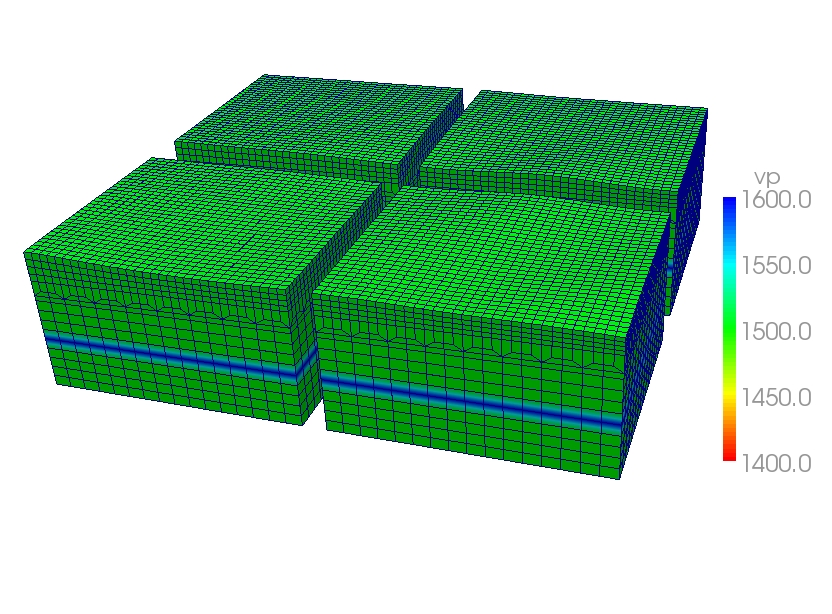
\includegraphics[width=.49\textwidth]{figures/vtk_mesh_vp.jpg}
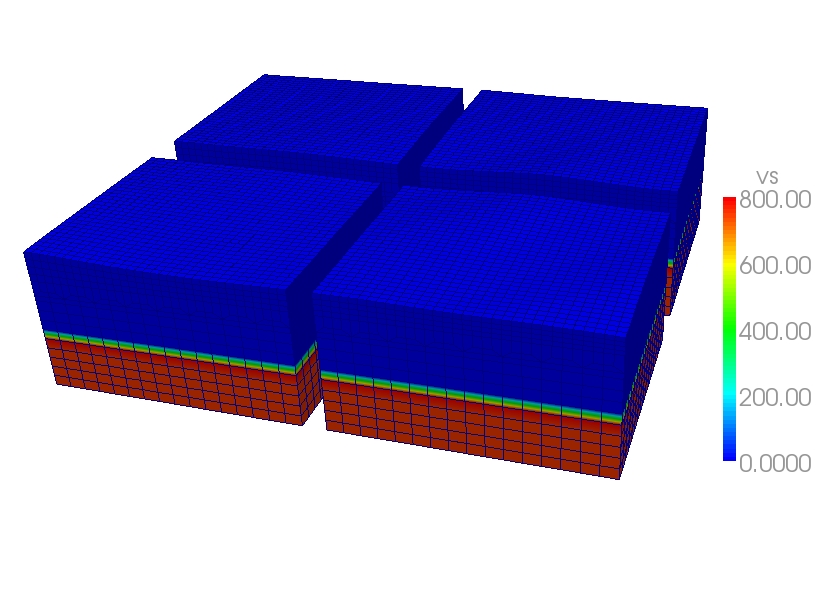
\includegraphics[width=.49\textwidth]{figures/vtk_mesh_vs.jpg}
\par\end{centering}

\caption{Visualization using Paraview of VTK files created by \texttt{xgenerate\_databases} showing P- and S-wave velocities assigned to the mesh points. The mesh was created by \texttt{xmeshfem3D} for 4 processors.}

\label{fig:vtk.mesh}
\end{figure}


You have also the option to visualize the distributed databases produced by \texttt{xgenerate\_databases}
using Paraview \url{www.paraview.org}. For this, you must set the flag \texttt{SAVE\_MESH\_FILES} to \texttt{.true.}
in the main parameter file \texttt{Par\_file} (see Chapter~\ref{cha:Main-Parameter} for details).
This will create VTK files for each single partition. You can then use Paraview \url{www.paraview.org} to visualized these partitions.


\section{\label{sec:Movies}Movies}

To make a surface or volume movie of the simulation, set parameters
\texttt{MOVIE\_SURFACE}, \texttt{MOVIE\_VOLUME}, and \texttt{NTSTEP\_BETWEEN\_FRAMES}
in the \texttt{Par\_file}. Turning on the movie flags, in particular
\texttt{MOVIE\_VOLUME}, produces large output files. \texttt{MOVIE\_VOLUME}
files are saved in the \texttt{LOCAL\_PATH} directory, whereas \texttt{MOVIE\_SURFACE}
output files are saved in the \texttt{in\_out\_files/OUTPUT\_FILES} directory. We
save the velocity field. The look of a movie is determined by the
half-duration of the source. The half-duration should be large enough
so that the movie does not contain frequencies that are not resolved
by the mesh, i.e., it should not contain numerical noise. This can
be accomplished by selecting a CMT \texttt{HALF\_DURATION} > 1.1 $\times$
smallest period (see figure \ref{fig:CMTSOLUTION-file}). When \texttt{MOVIE\_SURFACE}
= .\texttt{true.}, the half duration of each source in the \texttt{CMTSOLUTION}
file is replaced by

\begin{quote}
\[
\sqrt{(}\mathrm{\mathtt{HALF\_DURATIO}\mathtt{N}^{2}}+\mathrm{\mathtt{HDUR\_MOVI}\mathtt{E}^{2}})\]
\textbf{NOTE:} If \texttt{HDUR\_MOVIE} is set to 0.0, the code will
select the appropriate value of 1.1 $\times$ smallest period. As
usual, for a point source one can set \texttt{HALF\_DURATION} in the
\texttt{Par\_file} to be 0.0 and \texttt{HDUR\_MOVIE} = 0.0 to get
the highest frequencies resolved by the simulation, but for a finite
source one would keep all the \texttt{HALF\_DURATIONs} as prescribed
by the finite source model and set \texttt{HDUR\_MOVIE} = 0.0.
\end{quote}

\subsection{Movie Surface}

When running \texttt{xspecfem3D} with the \texttt{MOVIE\_SURFACE}
flag turned on, the code outputs \texttt{moviedata??????} files in
the \texttt{in\_out\_files/OUTPUT\_FILES} directory. The files are in a fairly complicated
binary format, but there is a program provided to convert the
output into more user friendly formats: 

\begin{description}
\item [\texttt{xcreate\_movie\_shakemap\_AVS\_DX\_GMT}] 
From \texttt{create\_movie\_shakemap\_AVS\_DX\_GMT.f90}, it
outputs data in ASCII, OpenDX, or AVS format (also readable in ParaView). 
Before compiling the code, make sure you have the file \texttt{surface\_from\_mesher.h}
in the  \texttt{in\_out\_files/OUTPUT\_FILES/} directory. This file will be created by the solver run.
Then type `\texttt{make} \texttt{create\_movie\_shakemap\_AVS\_DX\_GMT}'
and run the executable \texttt{xcreate\_movie\_shakemap\_AVS\_DX\_GMT}
in the \texttt{bin/} subdirectory. It will create visualization files in your format of choice. The code
will prompt the user for input parameters. 

\begin{figure}[htbp]
\noindent \begin{centering}
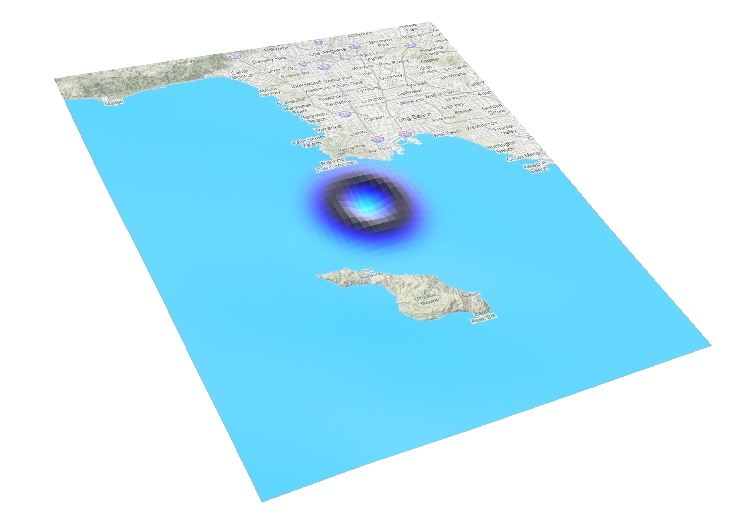
\includegraphics[width=.32\textwidth]{figures/movie_surf_1.jpg}
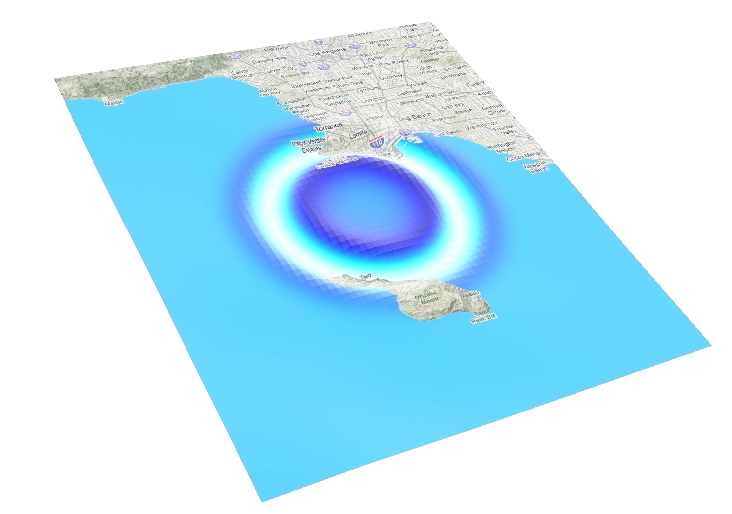
\includegraphics[width=.32\textwidth]{figures/movie_surf_2.jpg}
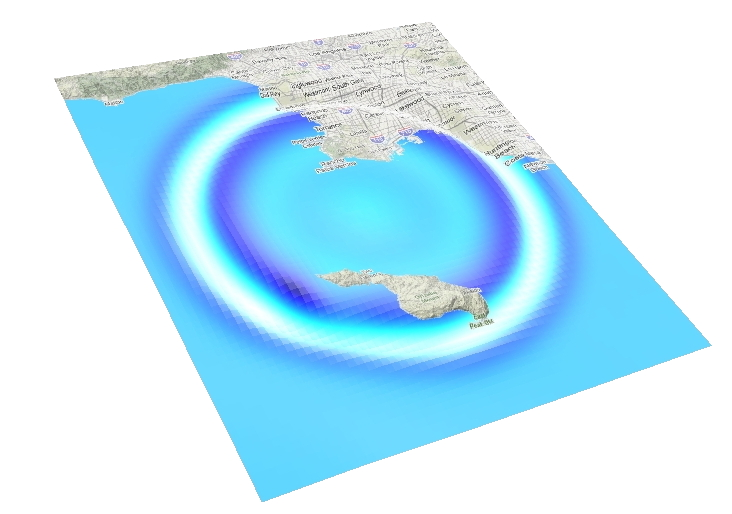
\includegraphics[width=.32\textwidth]{figures/movie_surf_3.jpg}
\par\end{centering}

\caption{Visualization using AVS files created by \texttt{xcreate\_movie\_shakemap\_AVS\_DX\_GMT} showing 
movie snapshots of vertical velocity components at different times.}

\label{fig:movie.surf}
\end{figure}

% uses obsolete routines...
%\item [\texttt{xcreate\_movie\_GMT}]
%From \texttt{create\_movie\_GMT.f90},
%outputs ascii xyz files, convenient for use with GMT. This code uses
%significantly less memory than \texttt{create\_movie\_shakemap\_AVS\_DX\_GMT.f90}
%and is therefore useful for high resolution runs.

\end{description}

The \texttt{SPECFEM3D} code is running in near real-time to produce
animations of southern California earthquakes via the web; see Southern California ShakeMovie\textregistered \url{www.shakemovie.caltech.edu}.


\section{\label{sec:Finite-Frequency-Kernels}Finite-Frequency Kernels}

The finite-frequency kernels computed as explained in Section \ref{sec:Adjoint-simulation-finite}
are saved in the \texttt{LOCAL\_PATH} at the end of the simulation.
Therefore, we first need to collect these files on the front end,
combine them into one mesh file, and visualize them with some auxilliary
programs.

\begin{enumerate}
\item \textbf{Create slice files}


We will only discuss the case of one source-receiver pair, i.e., the
so-called banana-doughnut kernels. Although it is possible to collect
the kernel files from all slices on the front end, it usually takes
up too much storage space (at least tens of gigabytes). Since the
sensitivity kernels are the strongest along the source-receiver great
circle path, it is sufficient to collect only the slices that are
along or close to the great circle path.

A Perl script \texttt{slice\_number.pl} located in directory \texttt{utils/Visualization/Paraview/} can
help to figure out the slice numbers that lie along the great circle
path. It applies to meshes created with the internal mesher \texttt{xmeshfem3D}.


\begin{enumerate}
\item On machines where you have access to the script, copy the \texttt{Mesh\_Par\_file}, and
\texttt{output\_solver} files, and run:

\begin{lyxcode}
{\small slice\_number.pl~Mesh\_Par\_file~output\_solver.txt~slice\_file}{\small \par}
\end{lyxcode}
which will generate a \texttt{slices\_file}.

\item For cases with multiple sources and multiple receivers, you need to
provide a slice file before proceeding to the next step.
\end{enumerate}
\item \textbf{Collect the kernel files}


After obtaining the slice files, you can collect the corresponding
kernel files from the given slices.

\begin{enumerate}
\item You can use or modify the script \texttt{utils/copy\_basin\_database.pl}
to accomplish this:

\begin{lyxcode}
{\small utils/copy\_database.pl~slice\_file~lsf\_machine\_file~filename~{[}jobid]}{\small \par}
\end{lyxcode}
where \texttt{\small lsf\_machine\_file} is the machine file generated
by the LSF scheduler, \texttt{\small filename} is the kernel name
(e.g., \texttt{\small rho\_kernel}, \texttt{\small alpha\_kernel}
and \texttt{\small beta\_kernel}), and the optional \texttt{\small jobid}
is the name of the subdirectory under \texttt{\small LOCAL\_PATH}
where all the kernel files are stored.

\item After executing this script, all the necessary mesh topology files
as well as the kernel array files are collected to the local directory
of the front end.
\end{enumerate}
\item \textbf{Combine kernel files into one mesh file}


We use an auxilliary program \texttt{combine\_vol\_data.f90}
to combine the kernel files from all slices into one mesh file.

\begin{enumerate}
\item Compile it in the root directory:

\begin{lyxcode}
{\footnotesize make~combine\_vol\_data~}{\footnotesize \par}

{\footnotesize ./bin/xcombine\_vol\_data~slice\_list~filename~input\_dir~output\_dir~high/low-resolution~}{\footnotesize \par}
\end{lyxcode}
where \texttt{input\_dir} is the directory where all the individual
kernel files are stored, and \texttt{output\_dir} is where the mesh
file will be written.

\item Use 1 for a high-resolution mesh, outputting all the GLL points to
the mesh file, or use 0 for low resolution, outputting only the corner
points of the elements to the mesh file.
\item The output mesh file will have the name \texttt{filename\_rho(alpha,beta).mesh}
\end{enumerate}
\item \textbf{Convert mesh files into .vtu files}

\begin{enumerate}
\item We next convert the \texttt{.mesh} file into the VTU (Unstructured
grid file) format which can be viewed in ParaView. For this task, you can use and modify the script \texttt{mesh2vtu.pl}
located in directory \texttt{utils/Visualization/Paraview/}, for example:

\begin{lyxcode}
mesh2vtu.pl~-i~file.mesh~-o~file.vtu
\end{lyxcode}
\item Notice that this Perl script uses a program \texttt{mesh2vtu} in the
\texttt{utils/Visualization/Paraview/mesh2vtu} directory, which further uses the VTK \url{http://www.vtk.org/}
run-time library for its execution. Therefore, make sure you have
them properly set in the script according to your system.
\end{enumerate}
\item \textbf{Copy over the source and receiver .vtk file}


In the case of a single source and a single receiver, the simulation
also generates the file \texttt{sr.vtk} located in the
\texttt{in\_out\_files/OUTPUT\_FILES/} directory to describe
the source and receiver locations, which can also be viewed in Paraview
in the next step.

\item \textbf{View the mesh in ParaView}


Finally, we can view the mesh in ParaView \url{www.paraview.org}.

\begin{enumerate}
\item Open ParaView.
\item From the top menu, \textsf{File} $\rightarrow$\textsf{Open data},
select \texttt{file.vtu}, and click the \textsf{Accept} button.

\begin{itemize}
\item If the mesh file is of moderate size, it shows up on the screen; otherwise,
only the bounding box is shown.
\end{itemize}
\item Click \textsf{Display Tab} $\rightarrow$ \textsf{Display Style} $\rightarrow$
\textsf{Representation} and select \textsf{wireframe of surface} to
display it.
\item To create a cross-section of the volumetric mesh, choose \textsf{Filter}
$\rightarrow$ \textsf{cut}, and under \textsf{Parameters Tab}, choose
\textsf{Cut Function} $\rightarrow$ \textsf{plane}.
\item Fill in center and normal information given by the \texttt{global\_slice\_number.pl}
script (either from the standard output or from \texttt{normal\_plane.txt}
file).
\item To change the color scale, go to \textsf{Display Tab} $\rightarrow$
\textsf{Color} $\rightarrow$ \textsf{Edit Color Map} and reselect
lower and upper limits, or change the color scheme.
\item Now load in the source and receiver location file by \textsf{File}
$\rightarrow$ \textsf{Open data}, select \texttt{sr.vt}k, and click
the \textsf{Accept} button. Choose \textsf{Filter} $\rightarrow$
\textsf{Glyph}, and represent the points by `\textsf{spheres}'.
\item For more information about ParaView, see the ParaView Users Guide \url{www.paraview.org/files/v1.6/ParaViewUsersGuide.PDF}.
\end{enumerate}
\end{enumerate}
%
\begin{figure}[H]
\noindent \begin{centering}
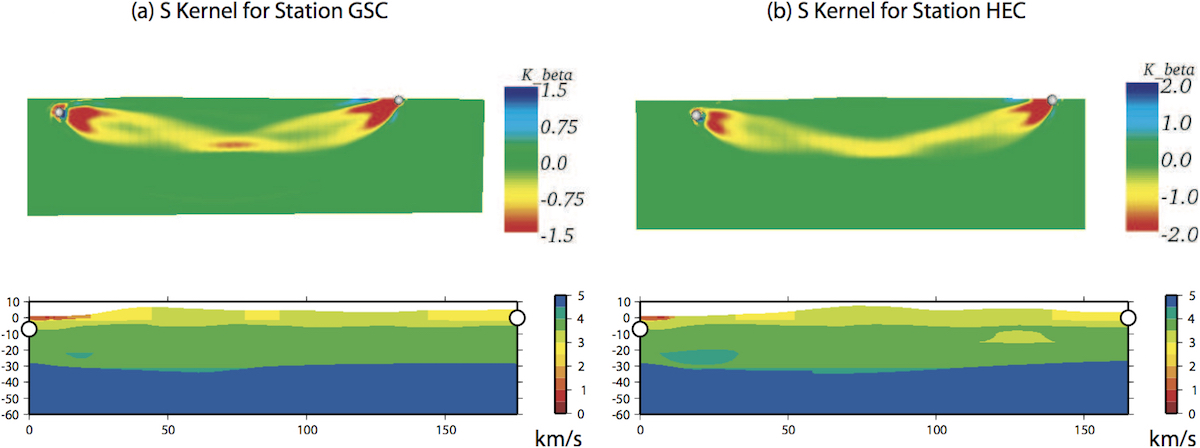
\includegraphics[scale=0.6]{figures/3D-S-Kernel}
\par\end{centering}

\caption{(a) Top Panel: Vertical source-receiver cross-section of the S-wave
finite-frequency sensitivity kernel $K_{\beta}$ for station GSC at
an epicentral distance of 176 km from the September 3, 2002, Yorba
Linda earthquake. Lower Panel: Vertical source-receiver cross-section
of the 3D S-wave speed model used for the spectral-element simulations
\citep{KoLiTrSuStSh04}. (b) The same as (a) but for station HEC at
an epicentral distance of 165 km \citep{LiTr06}.}


\label{figure:P-wave-speed-finite-frequency}
\end{figure}



\chapter{\label{cha:Scheduler}Running through a Scheduler}

The code is usually run on large parallel machines, often PC clusters,
most of which use schedulers, i.e., queuing or batch management systems
to manage the running of jobs from a large number of users. The following
considerations need to be taken into account when running on a system
that uses a scheduler:

\begin{itemize}
\item The processors/nodes to be used for each run are assigned dynamically
by the scheduler, based on availability. Therefore, in order for the
\texttt{xgenerate\_databases} and the \texttt{xspecfem3D} executables (or between successive runs of the solver) to
have access to the same database files (if they are stored on hard
drives local to the nodes on which the code is run), they must be
launched in sequence as a single job.
\item On some systems, the nodes to which running jobs are assigned are
not configured for compilation. It may therefore be necessary to pre-compile
both the \texttt{xgenerate\_databases} and the \texttt{xspecfem3D} executables.
%obsolete
%A small program provided in the distribution
%called \texttt{\small create\_header\_file.f90} can be used to directly
%create \texttt{\small in\_out\_files/OUTPUT\_FILES/values\_from\_mesher.h} using
%the information in the \texttt{\small in\_data\_files/Par\_file} without having
%to run the mesher (type \texttt{\small `make}{\small{} }\texttt{\small create\_header\_}~\\
%\texttt{\small file}' to compile it and `\texttt{\small xcreate\_header\_file}'
%to run it; refer to the sample scripts below). The solver can now
%be compiled as explained above.
\item One feature of schedulers/queuing systems is that they allow submission
of multiple jobs in a ``launch and forget'' mode. In order to take
advantage of this property, care needs to be taken that output and
intermediate files from separate jobs do not overwrite each other,
or otherwise interfere with other running jobs.
\end{itemize}
Examples of job scripts can be found in the \texttt{\small utils/Cluster/}
directory and can straightforwardly be modified and adapted to meet
more specific running needs.

We describe here in some detail a job submission procedure for the
Caltech 1024-node cluster, CITerra, under the LSF scheduling system.
We consider the submission of a regular forward simulation using the internal mesher
to create mesh partitions. The two
main scripts are \texttt{\small run\_lsf.bash}, which compiles the
Fortran code and submits the job to the scheduler, and \texttt{\small go\_mesher\_solver\_lsf\_basin.forward},
which contains the instructions that make up
the job itself. These scripts can be found in \texttt{\small utils/Cluster/lsf/} directory


\section{Job submission \texttt{run\_lsf.bash}}

This script first sets the job queue to be `normal'. It then compiles
the mesher, database generator and solver together, figures out the number of processors
required for this simulation from the \texttt{in\_data\_files/Par\_file}, and
submits the LSF job.

\begin{lyxcode}
\#!/bin/bash

\#~use~the~normal~queue~unless~otherwise~directed~queue=\char`\"{}-q~normal\char`\"{}~

if~{[}~\$\#~-eq~1~];~then

~~~~~~~~echo~\char`\"{}Setting~the~queue~to~\$1\char`\"{}

~~~~~~~~queue=\char`\"{}-q~\$1\char`\"{}~

fi~\\
~\\
\#~compile~the~mesher~and~the~solver~

d=`date'~echo~\char`\"{}Starting~compilation~\$d\char`\"{}~

make~clean~

make~meshfem3D~

make~generate\_databases~

make~specfem3D~

d=`date'~

echo~\char`\"{}Finished~compilation~\$d\char`\"{}~\\
~\\
\#~get~total~number~of~nodes~needed~for~solver~

NPROC=`grep~NPROC~in\_data\_files/Par\_file~|~cut~-c~34-~'~\\
~\\

\#~compute~total~number~of~nodes~needed~for~mesher~

NPROC\_XI=`grep~NPROC\_XI~in\_data\_files/meshfem3D\_files/Mesh\_Par\_file~|~cut~-c~34-~'~
~\\

NPROC\_ETA=`grep~NPROC\_ETA~in\_data\_files/meshfem3D\_files/Mesh\_Par\_file~|~cut~-c~34-~'~
~\\
\#~total~number~of~nodes~is~the~product~of~the~values~read~

numnodes=\$((~\$NPROC\_XI~*~\$NPROC\_ETA~))~\\
~\\

\#~checks~total~number~of~nodes~

if~{[}~\$numnodes~-neq~\$NPROC~];~then

~~~~~~~~echo~\char`\"{}error number of procs mismatch\char`\"{}

~~~~~~~~exit~

fi~\\

~\\
echo~\char`\"{}Submitting~job\char`\"{}~

bsub~\$queue~-n~\$numnodes~-W~60~-K~<go\_mesher\_solver\_lsf.forward~
\end{lyxcode}

\section{Job script \texttt{go\_mesher\_solver\_lsf.forward}}

This script describes the job itself, including setup steps that can
only be done once the scheduler has assigned a job-ID and a set of
compute nodes to the job, the \texttt{run\_lsf.bash} commands used
to run the mesher, database generator and the solver, and calls to scripts that collect
the output seismograms from the compute nodes and perform clean-up
operations.

\begin{enumerate}
\item First the script directs the scheduler to save its own output and
output from \texttt{stdout} into ~\\
\texttt{\small in\_out\_files/OUTPUT\_FILES/\%J.o},
where \texttt{\%J} is short-hand for the job-ID; it also tells the
scheduler what version of \texttt{mpich} to use (\texttt{mpich\_gm})
and how to name this job (\texttt{go\_mesher\_solver\_lsf}).
\item The script then creates a list of the nodes allocated to this job
by echoing the value of a dynamically set environment variable \texttt{LSB\_MCPU\_HOSTS}
and parsing the output into a one-column list using the Perl script
\texttt{utils/Cluster/lsf/remap\_lsf\_machines.pl}. It then creates a set of scratch
directories on these nodes (\texttt{\small /scratch/}~\\
\texttt{\small \$USER/DATABASES\_MPI}) to be used as the \texttt{LOCAL\_PATH}
for temporary storage of the database files. The scratch directories
are created using \texttt{shmux}, a shell multiplexor that can execute
the same commands on many hosts in parallel. \texttt{shmux} is available
from Shmux \url{web.taranis.org/shmux/}. Make sure that the \texttt{LOCAL\_PATH}
parameter in \texttt{in\_data\_files/Par\_file} is also set properly.
\item The next portion of the script launches the mesher, database generator and then the solver
using \texttt{run\_lsf.bash}.
\item The final portion of the script collects the seismograms and performs
clean up on the nodes, using the Perl scripts \texttt{collect\_seismo\_lsf\_multi.pl}
and \texttt{cleanmulti.pl}.
\end{enumerate}
\begin{lyxcode}
\#!/bin/bash~-v~

\#BSUB~-o~in\_out\_files/OUTPUT\_FILES/\%J.o~

\#BSUB~-a~mpich\_gm~

\#BSUB~-J~go\_mesher\_solver\_lsf~\\
~\\
\#~set~up~local~scratch~directories

BASEMPIDIR=/scratch/\$USER/DATABASES\_MPI

mkdir~-p~in\_out\_files/OUTPUT\_FILES~

echo~\char`\"{}\$LSB\_MCPU\_HOSTS\char`\"{}~>~in\_out\_files/OUTPUT\_FILES/lsf\_machines~

echo~\char`\"{}\$LSB\_JOBID\char`\"{}~>~in\_out\_files/OUTPUT\_FILES/jobid

remap\_lsf\_machines.pl~in\_out\_files/OUTPUT\_FILES/lsf\_machines~> in\_out\_files/OUTPUT\_FILES/machines

shmux~-M50~-Sall~-c~\char`\"{}rm~-r~-f~/scratch/\$USER;~\textbackslash{}

~~~~~~mkdir~-p~/scratch/\$USER;~mkdir~-p~\$BASEMPIDIR\char`\"{}~\textbackslash{}

~~~~~~-~<~in\_out\_files/OUTPUT\_FILES/machines~>/dev/null~\\
~\\
\#~run~the~specfem~program

current\_pwd=\$PWD \\

cd bin/ \\

run\_lsf.bash~-{}-gm-no-shmem~-{}-gm-copy-env~\$current\_pwd/xmeshfem3D~\\

run\_lsf.bash~-{}-gm-no-shmem~-{}-gm-copy-env~\$current\_pwd/xgenerate\_databases~\\

run\_lsf.bash~-{}-gm-no-shmem~-{}-gm-copy-env~\$current\_pwd/xspecfem3D~\\
~\\
\#~collect~seismograms~and~clean~up

cd current\_pwd/~ \\

mkdir~-p~in\_out\_files/SEM

cd~in\_out\_files/SEM/~

collect\_seismo.pl~../OUTPUT\_FILES/lsf\_machines

cleanbase.pl~../OUTPUT\_FILES/machines
\end{lyxcode}

\chapter{Post-Processing Scripts}

Several post-processing scripts/programs are provided in the \texttt{utils/}
directory, and most of them need to be adjusted when used on different
systems, for example, the path of the executable programs. Here we
only list a few of the available scripts and provide a brief description, and
you can either refer to the related sections for detailed usage or,
in a lot of cases, type the script/program name without arguments
for its usage.

\section{Process Data and Synthetics\label{sec:Process-data-and-syn}}

In many cases, the SEM synthetics are calculated and compared to data
seismograms recorded at seismic stations. Since the SEM synthetics
are accurate for a certain frequency range, both the original data
and the synthetics need to be processed before a comparison can be
made. We generally use the following scripts provided in the ~\\
\texttt{utils/seis\_process/} directory:


\subsection{Data processing script \texttt{process\_trinet\_data.pl}}

This script cuts a given portion of the original data, filters it,
transfers the data into a displacement record, and picks the first
P and S arrivals. For more functionality, type `\texttt{process\_trinet\_data.pl}'
without any argument. An example of the usage of the script:

\begin{lyxcode}
{\footnotesize process\_trinet\_data.pl~-m~CMTSOLUTION~-l~0/180~-t~2/40~-i~dir~-p~-x~bp~~9703873{*}.BH?.SAC}{\footnotesize \par}
\end{lyxcode}
which has cut all the sac files between 0 and 180 seconds, filtered
them between 2 and 40 seconds, transfered them into displacement records
using the polezero files in \texttt{dir} directory, picked the first
P and S arrivals, and added suffix `\texttt{bp}' to the file names.

Note that all of the scripts in this section actually use the SAC
and/or IASP91 to do the core operations; therefore make sure that
the SAC and IASP91 packages are installed properly on your system,
and that all the environment variables are set properly before running
these scripts.


\subsection{Synthetics processing script \texttt{process\_trinet\_syn.pl}}

This script converts the synthetic output from the SEM code from ASCII
to SAC format, and performs similar operations as `\texttt{process\_trinet\_data.pl}'.
An example of the usage of the script:

\begin{lyxcode}
{\footnotesize process\_trinet\_syn.pl~-m~CMTSOLUTION~-a~STATIONS~-l~0/180~-t~2/40~-p~-x~bp~syn/{*}.BH?.semd}{\footnotesize \par}
\end{lyxcode}
which will convert the synthetics into SAC format, add event and station
information into the SAC headers, cut the SAC files between 0 and
180 seconds, filter them between 2 and 40 seconds, pick the first
P and S arrivals, and add the suffix `\texttt{bp}' to the file names.

More options are available for this script, such as adding time shift
to the origin time of the synthetics, convolving the synthetics with
a triangular source time function with a given half duration, etc.
Type \texttt{process\_trinet\_syn.pl} without any argument for a detailed
usage.


\subsection{Script \texttt{rotate.pl}}

The original data and synthetics have three components: vertical (BHZ),
north (BHN) and east (BHE). However, for most seismology applications,
transverse and radial components are also desirable. Therefore, we
need to rotate the horizontal components of both the data and the
synthetics to the transverse and radial direction, and \texttt{\small rotate.pl}
can be used to accomplish this:

\begin{lyxcode}
rotate.pl~-l~0~-L~180~-d~DATA/{*}.BHE.SAC.bp~

rotate.pl~-l~0~-L~180~SEM/{*}.BHE.semd.sac.bp~
\end{lyxcode}
where the first command performs rotation on the SAC data obtained
through Seismogram Transfer Program (STP) \url{http://www.data.scec.org/STP/stp.html},
while the second command rotates the processed SEM synthetics.


\section{Collect Synthetic Seismograms}

The forward and adjoint simulations generate synthetic seismograms
in the \texttt{in\_out\_files/OUTPUT\_FILES/} directory by default. For the forward simulation, the files
are named \texttt{STA.NT.BH?.semd} for two-column time series, or
\texttt{STA.NT.BH?.semd.sac} for ASCII SAC format, where STA and NT
are the station name and network code, and \texttt{BH?} stands for
the component name. The adjont simulations generate synthetic seismograms
with the name \texttt{S?????.NT.S??.sem} (refer to Section \ref{sec:Adjoint-simulation-sources}
for details). The kernel simulations output the back-reconstructed
synthetic seismogram in the name \texttt{STA.NT.BH?.semd}, mainly
for the purpose of checking the accuracy of the reconstruction. Refer
to Section \ref{sec:Adjoint-simulation-finite} for further details.

You do have two options to change this default output behavior, given in the main constants file
\texttt{constants.h} located in \texttt{src/shared/} directory:
\begin{description}
\item [{\texttt{WRITE\_SEISMOGRAMS\_BY\_MASTER}}] Set to \texttt{.true.} to have only the master process writing out seismograms. This can be useful on a cluster, where only the master process node has access to the output directory.
\item [{\texttt{USE\_OUTPUT\_FILES\_PATH}}] Set to \texttt{.false.} to have the seismograms output to \texttt{LOCAL\_PATH} directory specified in the main parameter file \texttt{in\_data\_files/Par\_file}.
In this case, you could collect the synthetics onto the frontend using the \texttt{collect\_seismo\_lsf\_multi.pl} script
located in the \texttt{utils/Cluster/lsf/} directory. The usage of the script would be e.g.:

\begin{lyxcode}
collect\_seismo.pl~machines~in\_data\_files/Par\_file
\end{lyxcode}

\end{description}
where  \texttt{machines} is a file containing the node names and  \texttt{in\_data\_files/Par\_file} the parameter file used to extract the \texttt{LOCAL\_PATH} directory used for the simulation.


\section{Clean Local Database}

After all the simulations are done, the seismograms are collected,
and the useful database files are copied to the frontend, you may
need to clean the local scratch disk for the next simulation. This
is especially important in the case of kernel simulation,
where very large files are generated for the absorbing boundaries
to help with the reconstruction of the regular forward wavefield.
A sample script is provided in \texttt{utils/}:

\begin{lyxcode}
cleanbase.pl~machines
\end{lyxcode}
where  \texttt{machines} is a file containing the node names.

\section{Plot Movie Snapshots and Synthetic Shakemaps}


\subsection{\texttt{movie2gif.pl}}

With the movie data saved in \texttt{in\_out\_files/OUTPUT\_FILES/} at the end of
a movie simulation (\texttt{\small MOVIE\_SURFACE=.true.}), you can
run the \texttt{`create\_movie\_GMT}' code to convert these binary
movie data into GMT xyz files for futher processing. A sample script
\texttt{movie2gif.pl} is provided to do this conversion, and then
plot the movie snapshots in GMT, for example:

\begin{lyxcode}
movie2gif.pl~-m~CMTSOLUTION~-g~-f~1/40~-n~-2~-p~
\end{lyxcode}
which for the first through the 40th movie frame, converts the \texttt{moviedata}
files into GMT xyz files, interpolates them using the 'nearneighbor'
command in GMT, and plots them on a 2D topography map. Note that `\texttt{-2}'
and `\texttt{-p}' are both optional.


\subsection{\texttt{plot\_shakemap.pl}}

With the shakemap data saved in \texttt{in\_out\_files/OUTPUT\_FILES/} at the end
of a shakemap simulation ~\\
(\texttt{CREATE\_SHAKEMAP=.true.}), you can
also run \texttt{`create\_movie\_shakemap\_AVS\_DX\_GMT}' code to convert the binary
shakemap data into GMT xyz files. A sample script \texttt{plot\_shakemap.pl}
is provided to do this conversion, and then plot the shakemaps in
GMT, for example:

\begin{lyxcode}
plot\_shakemap.pl~data\_dir~type(1,2,3)~CMTSOLUTION~
\end{lyxcode}
where \texttt{type=1} for a displacement shakemap, \texttt{2} for
velocity, and \texttt{3} for acceleration.


\section{Map Local Database}

A sample program \texttt{remap\_database} is provided to map the local
database from a set of machines to another set of machines. This is
especially useful when you want to run mesher and solver, or different
types of solvers separately through a scheduler (refer to Chapter~\ref{cha:Scheduler}).

\begin{lyxcode}
run\_lsf.bash~-{}-gm-no-shmem~-{}-gm-copy-env~remap\_database~old\_machines~150
\end{lyxcode}
where \texttt{old\_machines} is the LSF machine file used in the previous
simulation, and \texttt{150} is the number of processors in total.


\chapter*{\label{cha:Bug-Reports-and}Bug Reports and Suggestions for Improvements}

To report bugs or suggest improvements to the code, please send an
e-mail to the CIG Computational Seismology Mailing List \url{cig-seismo@geodynamics.org}
or Jeroen Tromp \url{jtromp-AT-princeton.edu}, and/or use our online
bug tracking system Roundup \url{www.geodynamics.org/roundup}.


\chapter*{Notes \& Acknowledgments}

In order to keep the software package thread-safe in case a multithreaded
implementation of MPI is used, developers should not add modules or
common blocks to the source code but rather use regular subroutine
arguments (which can be grouped in ``derived types'' if needed for
clarity).

The Gauss-Lobatto-Legendre subroutines in \texttt{gll\_library.f90}
are based in part on software libraries from the Massachusetts Institute
of Technology, Department of Mechanical Engineering (Cambridge, Massachusetts, USA).
The non-structured global numbering software was provided by Paul
F. Fischer (Brown University, Providence, Rhode Island, USA, now at Argonne National Laboratory, USA).

OpenDX \url{http://www.opendx.org} is open-source based on IBM Data
Explorer, AVS \url{http://www.avs.com} is a trademark of Advanced
Visualization Systems, and ParaView \url{http://www.paraview.com}
is an open-source visualization platform.

%The main developers of the \texttt{SPECFEM3D} source code are Dimitri
%Komatitsch, Jeroen Tromp, and Qinya Liu. The following individuals
%(listed in alphabetical order) have also contributed to the development
%or improvement of the source code: Min Chen, Vala Hj\"orleifsd\'ottir,
%Jes\'us Labarta, and Leif Strand. The following individuals (listed in alphabetical
%order) contributed to this manual: Min Chen, Vala Hj\"orleifsd\'ottir,
%Sue Kientz, Dimitri Komatitsch, Qinya Liu, Alessia Maggi,
%Carl Tape, and Jeroen Tromp. The manual's cover graphic was created
%by Santiago Lombeyda from Caltech's Center for Advanced Computing Research (CACR) \url{http://www.cacr.caltech.edu}.
%Older versions of the code were initially developed by Dimitri Komatitsch at Institut de Physique du Globe (France)
%and then by Dimitri Komatitsch and Jeroen Tromp at Harvard University (USA).

Please e-mail your feedback, questions, comments, and suggestions
to Jeroen Tromp \url{jtromp-AT-princeton.edu} or to the CIG Computational Seismology Mailing List \url{cig-seismo@geodynamics.org}.


\chapter*{Copyright}

Main authors: Dimitri Komatitsch and Jeroen Tromp

Princeton University, USA,
and University of Pau / CNRS / INRIA, France

$\copyright$ Princeton University and University of Pau / CNRS / INRIA, February 2010

This program is free software; you can redistribute it and/or modify
it under the terms of the GNU General Public License as published
by the Free Software Foundation (see Appendix \ref{cha:License}).

\bibliography{bibliography}


\appendix

\chapter{\label{cha:Coordinates}Reference Frame Convention}

The code uses the following convention for the Cartesian reference
frame:

\begin{itemize}
\item the $x$ axis points East
\item the $y$ axis points North
\item the $z$ axis points up
\end{itemize}
Note that this convention is different from both the \citet{AkRi80}
convention and the Harvard Centroid-Moment Tensor (CMT) convention.
The Aki \& Richards convention is

\begin{itemize}
\item the $x$ axis points North
\item the $y$ axis points East
\item the $z$ axis points down
\end{itemize}
and the Harvard CMT convention is

\begin{itemize}
\item the $x$ axis points South
\item the $y$ axis points East
\item the $z$ axis points up
\end{itemize}

\chapter{\label{cha:License}License }

\textbf{GNU GENERAL PUBLIC LICENSE Version 2, June 1991. Copyright
(C) 1989, 1991 Free Software Foundation, Inc. 59 Temple Place, Suite
330, Boston, MA 02111-1307 USA} \\
Everyone is permitted to copy and distribute verbatim copies of this
license document, but changing it is not allowed.


\section*{Preamble}

The licenses for most software are designed to take away your freedom
to share and change it. By contrast, the GNU General Public License
is intended to guarantee your freedom to share and change free software
-- to make sure the software is free for all its users. This General
Public License applies to most of the Free Software Foundation's software
and to any other program whose authors commit to using it. (Some other
Free Software Foundation software is covered by the GNU Library General
Public License instead.) You can apply it to your programs, too.

When we speak of free software, we are referring to freedom, not price.
Our General Public Licenses are designed to make sure that you have
the freedom to distribute copies of free software (and charge for
this service if you wish), that you receive source code or can get
it if you want it, that you can change the software or use pieces
of it in new free programs; and that you know you can do these things.

To protect your rights, we need to make restrictions that forbid anyone
to deny you these rights or to ask you to surrender the rights. These
restrictions translate to certain responsibilities for you if you
distribute copies of the software, or if you modify it.

For example, if you distribute copies of such a program, whether gratis
or for a fee, you must give the recipients all the rights that you
have. You must make sure that they, too, receive or can get the source
code. And you must show them these terms so they know their rights.

We protect your rights with two steps:

\begin{enumerate}
\item Copyright the software, and
\item Offer you this license which gives you legal permission to copy, distribute
and/or modify the software.
\end{enumerate}
Also, for each author's protection and ours, we want to make certain
that everyone understands that there is no warranty for this free
software. If the software is modified by someone else and passed on,
we want its recipients to know that what they have is not the original,
so that any problems introduced by others will not reflect on the
original authors' reputations.

Finally, any free program is threatened constantly by software patents.
We wish to avoid the danger that redistributors of a free program
will individually obtain patent licenses, in effect making the program
proprietary. To prevent this, we have made it clear that any patent
must be licensed for everyone's free use or not licensed at all.

The precise terms and conditions for copying, distribution and modification
follow.


\section*{GNU GENERAL PUBLIC LICENSE TERMS AND CONDITIONS FOR COPYING, DISTRIBUTION
AND MODIFICATION }

\begin{itemize}

\item[0.]This License applies to any program or other work which
contains a notice placed by the copyright holder saying it may be
distributed under the terms of this General Public License. The ``Program''
below refers to any such program or work, and a ``work based on the
Program'' means either the Program or any derivative work under copyright
law: that is to say, a work containing the Program or a portion of
it, either verbatim or with modifications and/or translated into another
language. (Hereinafter, translation is included without limitation
in the term ``modification.'') Each licensee is addressed as ``you.''\\
\\
Activities other than copying, distribution and modification are not
covered by this License; they are outside its scope. The act of running
the Program is not restricted, and the output from the Program is
covered only if its contents constitute a work based on the Program
(independent of having been made by running the Program). Whether
that is true depends on what the Program does.

\end{itemize}

\begin{enumerate}
\item You may copy and distribute verbatim copies of the Program's source
code as you receive it, in any medium, provided that you conspicuously
and appropriately publish on each copy an appropriate copyright notice
and disclaimer of warranty; keep intact all the notices that refer
to this License and to the absence of any warranty; and give any other
recipients of the Program a copy of this License along with the Program.


You may charge a fee for the physical act of transferring a copy,
and you may at your option offer warranty protection in exchange for
a fee.

\item You may modify your copy or copies of the Program or any portion of
it, thus forming a work based on the Program, and copy and distribute
such modifications or work under the terms of Section 1 above, provided
that you also meet all of these conditions:

\begin{enumerate}
\item You must cause the modified files to carry prominent notices stating
that you changed the files and the date of any change.
\item You must cause any work that you distribute or publish, that in whole
or in part contains or is derived from the Program or any part thereof,
to be licensed as a whole at no charge to all third parties under
the terms of this License.
\item If the modified program normally reads commands interactively when
run, you must cause it, when started running for such interactive
use in the most ordinary way, to print or display an announcement
including an appropriate copyright notice and a notice that there
is no warranty (or else, saying that you provide a warranty) and that
users may redistribute the program under these conditions, and telling
the user how to view a copy of this License. (Exception: if the Program
itself is interactive but does not normally print such an announcement,
your work based on the Program is not required to print an announcement.)
\end{enumerate}
These requirements apply to the modified work as a whole. If identifiable
sections of that work are not derived from the Program, and can be
reasonably considered independent and separate works in themselves,
then this License, and its terms, do not apply to those sections when
you distribute them as separate works. But when you distribute the
same sections as part of a whole which is a work based on the Program,
the distribution of the whole must be on the terms of this License,
whose permissions for other licensees extend to the entire whole,
and thus to each and every part regardless of who wrote it.

Thus, it is not the intent of this section to claim rights or contest
your rights to work written entirely by you; rather, the intent is
to exercise the right to control the distribution of derivative or
collective works based on the Program.

In addition, mere aggregation of another work not based on the Program
with the Program (or with a work based on the Program) on a volume
of a storage or distribution medium does not bring the other work
under the scope of this License.

\item You may copy and distribute the Program (or a work based on it, under
Section 2) in object code or executable form under the terms of Sections
1 and 2 above provided that you also do one of the following:

\begin{enumerate}
\item Accompany it with the complete corresponding machine-readable source
code, which must be distributed under the terms of Sections 1 and
2 above on a medium customarily used for software interchange; or,
\item Accompany it with a written offer, valid for at least three years,
to give any third party, for a charge no more than your cost of physically
performing source distribution, a complete machine-readable copy of
the corresponding source code, to be distributed under the terms of
Sections 1 and 2 above on a medium customarily used for software interchange;
or,
\item Accompany it with the information you received as to the offer to
distribute corresponding source code. (This alternative is allowed
only for noncommercial distribution and only if you received the program
in object code or executable form with such an offer, in accord with
Subsection b above.)
\end{enumerate}
The source code for a work means the preferred form of the work for
making modifications to it. For an executable work, complete source
code means all the source code for all modules it contains, plus any
associated interface definition files, plus the scripts used to control
compilation and installation of the executable. However, as a special
exception, the source code distributed need not include anything that
is normally distributed (in either source or binary form) with the
major components (compiler, kernel, and so on) of the operating system
on which the executable runs, unless that component itself accompanies
the executable.

If distribution of executable or object code is made by offering access
to copy from a designated place, then offering equivalent access to
copy the source code from the same place counts as distribution of
the source code, even though third parties are not compelled to copy
the source along with the object code.

\item You may not copy, modify, sublicense, or distribute the Program except
as expressly provided under this License. Any attempt otherwise to
copy, modify, sublicense or distribute the Program is void, and will
automatically terminate your rights under this License. However, parties
who have received copies, or rights, from you under this License will
not have their licenses terminated so long as such parties remain
in full compliance.
\item You are not required to accept this License, since you have not signed
it. However, nothing else grants you permission to modify or distribute
the Program or its derivative works. These actions are prohibited
by law if you do not accept this License. Therefore, by modifying
or distributing the Program (or any work based on the Program), you
indicate your acceptance of this License to do so, and all its terms
and conditions for copying, distributing or modifying the Program
or works based on it.
\item Each time you redistribute the Program (or any work based on the Program),
the recipient automatically receives a license from the original licensor
to copy, distribute or modify the Program subject to these terms and
conditions. You may not impose any further restrictions on the recipients'
exercise of the rights granted herein. You are not responsible for
enforcing compliance by third parties to this License.
\item If, as a consequence of a court judgment or allegation of patent infringement
or for any other reason (not limited to patent issues), conditions
are imposed on you (whether by court order, agreement or otherwise)
that contradict the conditions of this License, they do not excuse
you from the conditions of this License. If you cannot distribute
so as to satisfy simultaneously your obligations under this License
and any other pertinent obligations, then as a consequence you may
not distribute the Program at all. For example, if a patent license
would not permit royalty-free redistribution of the Program by all
those who receive copies directly or indirectly through you, then
the only way you could satisfy both it and this License would be to
refrain entirely from distribution of the Program.


If any portion of this section is held invalid or unenforceable under
any particular circumstance, the balance of the section is intended
to apply and the section as a whole is intended to apply in other
circumstances.

It is not the purpose of this section to induce you to infringe any
patents or other property right claims or to contest validity of any
such claims; this section has the sole purpose of protecting the integrity
of the free software distribution system, which is implemented by
public license practices. Many people have made generous contributions
to the wide range of software distributed through that system in reliance
on consistent application of that system; it is up to the author/donor
to decide if he or she is willing to distribute software through any
other system and a licensee cannot impose that choice.

This section is intended to make thoroughly clear what is believed
to be a consequence of the rest of this License.

\item If the distribution and/or use of the Program is restricted in certain
countries either by patents or by copyrighted interfaces, the original
copyright holder who places the Program under this License may add
an explicit geographical distribution limitation excluding those countries,
so that distribution is permitted only in or among countries not thus
excluded. In such case, this License incorporates the limitation as
if written in the body of this License.
\item The Free Software Foundation may publish revised and/or new versions
of the General Public License from time to time. Such new versions
will be similar in spirit to the present version, but may differ in
detail to address new problems or concerns.


Each version is given a distinguishing version number. If the Program
specifies a version number of this License which applies to it and
``any later version,'' you have the option of following the terms
and conditions either of that version or of any later version published
by the Free Software Foundation. If the Program does not specify a
version number of this License, you may choose any version ever published
by the Free Software Foundation.

\item If you wish to incorporate parts of the Program into other free programs
whose distribution conditions are different, write to the author to
ask for permission. For software which is copyrighted by the Free
Software Foundation, write to the Free Software Foundation; we sometimes
make exceptions for this. Our decision will be guided by the two goals
of preserving the free status of all derivatives of our free software
and of promoting the sharing and reuse of software generally.
\end{enumerate}

\subsection*{NO WARRANTY }

\begin{itemize}

\item[11.]BECAUSE THE PROGRAM IS LICENSED FREE OF CHARGE, THERE IS
NO WARRANTY FOR THE PROGRAM, TO THE EXTENT PERMITTED BY APPLICABLE
LAW. EXCEPT WHEN OTHERWISE STATED IN WRITING THE COPYRIGHT HOLDERS
AND/OR OTHER PARTIES PROVIDE THE PROGRAM ``AS IS'' WITHOUT WARRANTY
OF ANY KIND, EITHER EXPRESSED OR IMPLIED, INCLUDING, BUT NOT LIMITED
TO, THE IMPLIED WARRANTIES OF MERCHANTABILITY AND FITNESS FOR A PARTICULAR
PURPOSE. THE ENTIRE RISK AS TO THE QUALITY AND PERFORMANCE OF THE
PROGRAM IS WITH YOU. SHOULD THE PROGRAM PROVE DEFECTIVE, YOU ASSUME
THE COST OF ALL NECESSARY SERVICING, REPAIR OR CORRECTION.

\item[12.]IN NO EVENT UNLESS REQUIRED BY APPLICABLE LAW OR AGREED
TO IN WRITING WILL ANY COPYRIGHT HOLDER, OR ANY OTHER PARTY WHO MAY
MODIFY AND/OR REDISTRIBUTE THE PROGRAM AS PERMITTED ABOVE, BE LIABLE
TO YOU FOR DAMAGES, INCLUDING ANY GENERAL, SPECIAL, INCIDENTAL OR
CONSEQUENTIAL DAMAGES ARISING OUT OF THE USE OR INABILITY TO USE THE
PROGRAM (INCLUDING BUT NOT LIMITED TO LOSS OF DATA OR DATA BEING RENDERED
INACCURATE OR LOSSES SUSTAINED BY YOU OR THIRD PARTIES OR A FAILURE
OF THE PROGRAM TO OPERATE WITH ANY OTHER PROGRAMS), EVEN IF SUCH HOLDER
OR OTHER PARTY HAS BEEN ADVISED OF THE POSSIBILITY OF SUCH DAMAGES.

\end{itemize}


\section*{END OF TERMS AND CONDITIONS }


\subsection*{How to Apply These Terms to Your New Programs}

If you develop a new program, and you want it to be of the greatest
possible use to the public, the best way to achieve this is to make
it free software which everyone can redistribute and change under
these terms.

To do so, attach the following notices to the program. It is safest
to attach them to the start of each source file to most effectively
convey the exclusion of warranty; and each file should have at least
the ``copyright'' line and a pointer to where the full notice is found.
For example:

\begin{quote}
One line to give the program's name and a brief idea of what it does.
Copyright {\footnotesize $\copyright$ (}year) (name of author)

This program is free software; you can redistribute it and/or modify
it under the terms of the GNU General Public License as published
by the Free Software Foundation; either version 2 of the License,
or (at your option) any later version.

This program is distributed in the hope that it will be useful, but
WITHOUT ANY WARRANTY; without even the implied warranty of MERCHANTABILITY
or FITNESS FOR A PARTICULAR PURPOSE. See the GNU General Public License
for more details.

You should have received a copy of the GNU General Public License
along with this program; if not, write to the Free Software Foundation,
Inc., 59 Temple Place, Suite 330, Boston, MA 02111-1307 USA
\end{quote}
Also add information on how to contact you by electronic and paper
mail.

If the program is interactive, make it output a short notice like
this when it starts in an interactive mode:

\begin{quote}
Gnomovision version 69, Copyright $\copyright$ year name of author Gnomovision
comes with ABSOLUTELY NO WARRANTY; for details type `show w'. This
is free software, and you are welcome to redistribute it under certain
conditions; type `show c' for details.
\end{quote}
The hypothetical commands `show w' and `show c' should show the appropriate
parts of the General Public License. Of course, the commands you use
may be called something other than `show w' and `show c'; they could
even be mouse-clicks or menu items -- whatever suits your program.

You should also get your employer (if you work as a programmer) or
your school, if any, to sign a ``copyright disclaimer'' for the program,
if necessary. Here is a sample; alter the names:

\begin{quote}
Yoyodyne, Inc., hereby disclaims all copyright interest in the program
`Gnomovision' (which makes passes at compilers) written by James Hacker.

(signature of Ty Coon)\\
1 April 1989 \\
Ty Coon, President of Vice
\end{quote}
This General Public License does not permit incorporating your program
into proprietary programs. If your program is a subroutine library,
you may consider it more useful to permit linking proprietary applications
with the library. If this is what you want to do, use the GNU Library
General Public License instead of this License.
\end{document}
